\documentclass[12pt,a4paper]{article}

\usepackage{fontspec}
\usepackage{polyglossia}
\setdefaultlanguage{greek}
\setotherlanguage{english}

\setmainfont{Times New Roman}
\setsansfont{Arial}
\setmonofont{Consolas}
\newfontfamily\greekfonttt[Script=Greek]{Consolas}

\usepackage{geometry}
\usepackage{graphicx}
\usepackage{float}
\usepackage{caption}
\usepackage{xcolor}
\usepackage{listings}
\usepackage{amsmath}
\usepackage[hidelinks]{hyperref}
\usepackage{fancyhdr}
\usepackage{tikz}
\usetikzlibrary{arrows.meta}

\geometry{left=2.5cm,right=2.5cm,top=2.5cm,bottom=2.5cm}

\definecolor{codegreen}{rgb}{0,0.6,0}
\definecolor{codegray}{rgb}{0.5,0.5,0.5}
\definecolor{backcolour}{rgb}{0.95,0.95,0.92}

\lstset{
    backgroundcolor=\color{backcolour},
    commentstyle=\color{codegreen},
    keywordstyle=\color{blue},
    basicstyle=\ttfamily\small,
    breaklines=true,
    numbers=left,
    numberstyle=\tiny\color{codegray},
    language=Python,
    frame=single
}

\pagestyle{fancy}
\fancyhf{}
\rhead{AEM: 6931 -- Ρακοβαλής Παύλος}
\lhead{Data Analysis 2025-26}
\cfoot{\thepage}

\title{
    \textbf{Ανάλυση Δεδομένων 2025-26}\\[0.3cm]
    \large 1η Εργασία: Ανάλυση Ποιότητας Κρασιού\\[0.2cm]
    \normalsize AEM: 6931 -- Ρακοβαλής Παύλος
}
\author{}
\date{Μάρτιος 2026}

\begin{document}
\maketitle
\tableofcontents
\newpage

\section{Ερώτημα 1: Δειγματοληψία και Καθαρισμός Δεδομένων}

\subsection{Εισαγωγή}

\subsubsection{Σκοπός της Εργασίας}

Η παρούσα εργασία αφορά την ανάλυση δεδομένων ποιότητας κρασιού. Οι στόχοι είναι:

\begin{enumerate}
    \item Επιλογή τυχαίου δείγματος 80\% με seed τον ΑΕΜ
    \item Έλεγχος ποιότητας δεδομένων
    \item Καθαρισμός δεδομένων
\end{enumerate}

\subsubsection{Τι είναι ο Καθαρισμός Δεδομένων;}

\textbf{Ορισμός:} Ο καθαρισμός δεδομένων είναι η διαδικασία εντοπισμού και διόρθωσης λανθασμένων, ελλιπών, διπλότυπων ή ασυνεπών εγγραφών. Είναι κρίσιμο βήμα πριν από οποιαδήποτε ανάλυση.

Συνήθη προβλήματα:
\begin{itemize}
    \item \textbf{Τυπογραφικά λάθη:} π.χ. ``whte'' αντί ``white''
    \item \textbf{Ελλείπουσες τιμές:} Κενά πεδία
    \item \textbf{Μη έγκυρες τιμές:} π.χ. pH = 999
    \item \textbf{Διπλοεγγραφές:} Επαναλαμβανόμενες γραμμές
\end{itemize}

\subsection{Περιγραφή Δεδομένων}

\subsubsection{Μεταβλητές}

Το dataset περιέχει τις εξής μεταβλητές:

\begin{enumerate}
    \item \textbf{Fixed acidity} - Σταθερή οξύτητα (g/L)
    \item \textbf{Volatile acidity} - Πτητική οξύτητα (g/L)
    \item \textbf{Citric acid} - Κιτρικό οξύ (g/L)
    \item \textbf{Residual sugar} - Υπολειμματικά σάκχαρα (g/L)
    \item \textbf{Chlorides} - Χλωριούχα άλατα (g/L)
    \item \textbf{Free SO2} - Ελεύθερο διοξείδιο του θείου (mg/L)
    \item \textbf{Total SO2} - Συνολικό διοξείδιο του θείου (mg/L)
    \item \textbf{Density} - Πυκνότητα (g/cm3)
    \item \textbf{pH} - Οξύτητα (κλίμακα 2-14)
    \item \textbf{Sulphates} - Θειικά άλατα (g/L)
    \item \textbf{Alcohol} - Περιεκτικότητα σε αλκοόλ (\%)
    \item \textbf{Quality} - Βαθμολογία ποιότητας (0-10)
    \item \textbf{Wine\_type} - Τύπος κρασιού (red ή white)
\end{enumerate}

Αρχικό dataset: \textbf{8.385} γραμμές $\times$ \textbf{15} στήλες

\subsection{Δειγματοληψία}

\subsubsection{Τι είναι το Seed και γιατί το χρησιμοποιούμε;}

Το \textbf{seed} (σπόρος) είναι ένας αριθμός που αρχικοποιεί τη \textbf{γεννήτρια τυχαίων αριθμών} του υπολογιστή.

\textbf{Το πρόβλημα χωρίς seed:}

Οι υπολογιστές δεν μπορούν να παράγουν πραγματικά τυχαίους αριθμούς. Αντί αυτού, χρησιμοποιούν μαθηματικούς αλγορίθμους που παράγουν \textbf{ψευδοτυχαίους αριθμούς} (pseudo-random numbers) -- ακολουθίες αριθμών που φαίνονται τυχαίες αλλά στην πραγματικότητα είναι ντετερμινιστικές.

Αν δεν ορίσουμε seed, κάθε φορά που τρέχουμε τον κώδικα παίρνουμε διαφορετικό δείγμα:

\begin{lstlisting}
# Without seed - different results each time
sample1 = df.sample(frac=0.80)  # rows [5, 12, 3, 99, ...]
sample2 = df.sample(frac=0.80)  # rows [7, 45, 2, 88, ...]  <- Different!
\end{lstlisting}

\textbf{Η λύση με seed:}

Όταν ορίζουμε seed, ο αλγόριθμος ξεκινάει πάντα από το ίδιο σημείο και παράγει την ίδια ακολουθία ``τυχαίων'' αριθμών:

\begin{lstlisting}
# With seed - same results every time
sample1 = df.sample(frac=0.80, random_state=6931)  # rows [23, 45, 12, ...]
sample2 = df.sample(frac=0.80, random_state=6931)  # rows [23, 45, 12, ...] <- Same!
\end{lstlisting}

\textbf{Πώς λειτουργεί:}

$$\text{seed} = 6931 \xrightarrow{\text{αλγόριθμος}} [0.234, 0.891, 0.456, 0.123, \ldots] \text{ (πάντα η ίδια ακολουθία)}$$

\textbf{Γιατί χρησιμοποιούμε τον ΑΕΜ ως seed:}

\begin{enumerate}
    \item \textbf{Αναπαραγωγιμότητα (Reproducibility):} Ο καθηγητής μπορεί να τρέξει τον ίδιο κώδικα με το ίδιο seed και να επαληθεύσει τα αποτελέσματα
    \item \textbf{Μοναδικότητα:} Κάθε φοιτητής έχει διαφορετικό ΑΕΜ, άρα εργάζεται με διαφορετικό δείγμα δεδομένων
    \item \textbf{Επαλήθευση:} Αν χρειαστεί να ξανατρέξουμε την ανάλυση, θα πάρουμε ακριβώς τα ίδια δεδομένα
\end{enumerate}

\subsubsection{Εφαρμογή Δειγματοληψίας}

Χρησιμοποιούμε \textbf{seed = AEM = 6931}:

\begin{lstlisting}
import pandas as pd

df_original = pd.read_csv('Data Analysis_2026.csv')
AEM = 6931  # Our unique seed
df = df_original.sample(frac=0.80, random_state=AEM)
df = df.reset_index(drop=True)
\end{lstlisting}

\textbf{Τι κάνει κάθε γραμμή:}
\begin{itemize}
    \item \texttt{sample(frac=0.80)}: Επιλέγει τυχαία το 80\% των γραμμών
    \item \texttt{random\_state=AEM}: Ορίζει το seed ώστε το δείγμα να είναι αναπαραγώγιμο
    \item \texttt{reset\_index(drop=True)}: Επαναριθμεί τις γραμμές από 0 (αφαιρεί τους παλιούς αριθμούς)
\end{itemize}

\textbf{Αποτέλεσμα:} 8.385 $\rightarrow$ \textbf{6.708} γραμμές (80\%)

\subsection{Εντοπισμός Προβλημάτων}

\subsubsection{Τυπογραφικά Λάθη (wine\_type)}

Εντοπίστηκαν τα εξής λανθασμένα values στη στήλη wine\_type:

\begin{itemize}
    \item ``Redd '' (75 εγγραφές) $\rightarrow$ red
    \item ``whit'' (90 εγγραφές) $\rightarrow$ white
    \item ``r3d'' (64 εγγραφές) $\rightarrow$ red
    \item ``WHITTE'' (77 εγγραφές) $\rightarrow$ white
    \item ``whate'' (39 εγγραφές) $\rightarrow$ white
    \item 999, 9999, -999, ? (215 εγγραφές) $\rightarrow$ NaN
\end{itemize}

\textbf{Σύνολο τυπογραφικών λαθών:} 560

\subsubsection{Μη Αριθμητικές Τιμές}

Βρέθηκαν μη αριθμητικές τιμές (π.χ. ``abc'', ``?'', ``N/A'') στις αριθμητικές στήλες:

\begin{itemize}
    \item fixed acidity: 87 μη αριθμητικές τιμές
    \item volatile acidity: 45
    \item citric acid: 61
    \item pH: 151
    \item alcohol: 105
    \item κ.ά.
\end{itemize}

\textbf{Σύνολο μη αριθμητικών τιμών:} 845

\subsubsection{Αδύνατες Τιμές}

Τιμές όπως 999, -999, 9999 χρησιμοποιούνται συχνά ως κωδικοί για ελλείπουσες τιμές. Επίσης, κάποιες τιμές είναι εκτός λογικών ορίων (π.χ. pH = 999 ενώ το pH κυμαίνεται μεταξύ 0-14).

Λογικά όρια:
\begin{itemize}
    \item Fixed acidity: 0-20 g/L
    \item Volatile acidity: 0-5 g/L
    \item pH: 2-5
    \item Alcohol: 5-20\%
    \item Quality: 0-10
    \item Density: 0.9-1.1 g/cm$^3$
\end{itemize}

\textbf{Τιμές εκτός ορίων:} 2.037

\subsubsection{Διπλοεγγραφές}

\begin{lstlisting}
duplicates = df.duplicated()
print(f"Duplicates found: {duplicates.sum()}")
\end{lstlisting}

Εντοπίστηκαν \textbf{1.434} διπλοεγγραφές.

\subsubsection{Ελλείπουσες Τιμές (Missing Values)}

Μετά τη μετατροπή των μη αριθμητικών και αδύνατων τιμών σε NaN, οι ελλείπουσες τιμές ανά στήλη είναι:

\begin{itemize}
    \item fixed acidity: 574 (10.9\%)
    \item volatile acidity: 542 (10.3\%)
    \item density: 545 (10.3\%)
    \item pH: 644 (12.2\%)
    \item alcohol: 600 (11.4\%)
    \item quality: 40 (0.8\%)
\end{itemize}

\textbf{Σύνολο ελλειπουσών τιμών:} 3.092

\subsection{Αντιμετώπιση Προβλημάτων}

\subsubsection{Στρατηγική Αντιμετώπισης}

\begin{enumerate}
    \item \textbf{Τυπογραφικά λάθη wine\_type:} Διόρθωση στη σωστή τιμή ή NaN
    \item \textbf{Μη αριθμητικές τιμές:} Μετατροπή σε NaN
    \item \textbf{Αδύνατες τιμές:} Μετατροπή σε NaN
    \item \textbf{Διπλοεγγραφές:} Αφαίρεση
    \item \textbf{Missing values:} Συμπλήρωση με διάμεσο ανά τύπο κρασιού
\end{enumerate}

\subsubsection{Διόρθωση Τυπογραφικών Λαθών}

\begin{lstlisting}
corrections = {
    'Redd ': 'red', 'r3d': 'red',
    'WHITTE': 'white', 'whit': 'white', 'whate': 'white',
    '999': None, '9999': None, '-999': None, '?': None
}
for wrong, correct in corrections.items():
    df.loc[df['wine_type'] == wrong, 'wine_type'] = correct
\end{lstlisting}

\subsubsection{Γιατί Διάμεσος (Median) και όχι Μέσος Όρος;}

Η διάμεσος είναι η τιμή που χωρίζει τα δεδομένα στη μέση (50\% πάνω, 50\% κάτω). Είναι πιο ανθεκτική σε ακραίες τιμές (outliers) σε αντίθεση με τον μέσο όρο.

Παράδειγμα: Για τιμές [1, 2, 3, 4, 100]:
\begin{itemize}
    \item Μέσος όρος = 22 (επηρεάζεται από το 100)
    \item Διάμεσος = 3 (δεν επηρεάζεται)
\end{itemize}

\subsubsection{Γιατί ανά Τύπο Κρασιού;}

Τα κόκκινα και λευκά κρασιά έχουν διαφορετικά χημικά χαρακτηριστικά:

\begin{itemize}
    \item Κόκκινο - Fixed acidity (διάμεσος): 7.80
    \item Λευκό - Fixed acidity (διάμεσος): 6.80
    \item Κόκκινο - Total SO2 (διάμεσος): 40
    \item Λευκό - Total SO2 (διάμεσος): 133
\end{itemize}

\subsection{Αποτελέσματα}

\subsubsection{Συνοπτικός Πίνακας Προβλημάτων}

\begin{enumerate}
    \item Περιττές στήλες (Unnamed): 2 - Αφαιρέθηκαν
    \item Τυπογραφικά λάθη wine\_type: 560 - Διορθώθηκαν
    \item Μη αριθμητικές τιμές: 845 - Έγιναν NaN
    \item Αδύνατες τιμές: 2.037 - Έγιναν NaN
    \item Διπλοεγγραφές: 1.434 - Αφαιρέθηκαν
    \item Missing values (αρχικά): 3.092 - Συμπληρώθηκαν με διάμεσο
    \item Missing values (τελικά): 0
\end{enumerate}

\subsubsection{Εξέλιξη Μεγέθους Dataset}

\begin{enumerate}
    \item Αρχικό: 8.385 γραμμές × 15 στήλες
    \item Μετά sample (80\%): 6.708 γραμμές × 13 στήλες
    \item Μετά αφαίρεση duplicates: 5.274 γραμμές × 13 στήλες
    \item \textbf{Τελικό: 5.274 γραμμές × 13 στήλες}
\end{enumerate}

\subsubsection{Κατανομή Τελικού Dataset}

\begin{itemize}
    \item Λευκό κρασί: 3.924 (74.4\%)
    \item Κόκκινο κρασί: 1.350 (25.6\%)
    \item \textbf{Σύνολο: 5.274 (100\%)}
\end{itemize}

\subsection{Συμπεράσματα}

\begin{enumerate}
    \item Τα πραγματικά δεδομένα περιέχουν πολλαπλά προβλήματα ποιότητας
    \item Ο καθαρισμός δεδομένων είναι απαραίτητος πριν από κάθε ανάλυση
    \item Κάθε τύπος προβλήματος απαιτεί διαφορετική αντιμετώπιση
    \item Οι αποφάσεις καθαρισμού πρέπει να είναι τεκμηριωμένες
    \item Η χρήση seed εξασφαλίζει αναπαραγωγιμότητα
\end{enumerate}

Το καθαρισμένο dataset αποθηκεύτηκε στο αρχείο: \texttt{cleaned\_wine\_data\_AEM\_6931.csv}

%=============================================================================
% ΕΡΩΤΗΜΑ 2: BOXPLOTS
%=============================================================================
\newpage
\section{Ερώτημα 2: Γραφήματα Boxplot}

\subsection{Τι είναι το Boxplot;}

Το \textbf{boxplot} (ή box-and-whisker plot) είναι ένα γράφημα που απεικονίζει την κατανομή μιας αριθμητικής μεταβλητής με τρόπο συνοπτικό αλλά πλούσιο σε πληροφορίες. Εφευρέθηκε από τον στατιστικολόγο John Tukey το 1970.

\subsection{Τα Στοιχεία του Boxplot}

Ένα boxplot αποτελείται από τα εξής στοιχεία:

\begin{figure}[H]
\centering
\begin{tikzpicture}[x=1cm,y=1cm,>=Latex]
    % Box
    \draw[thick, fill=blue!10] (0,0) rectangle (2,3);
    % Median
    \draw[ultra thick, red] (0,1.5) -- (2,1.5);
    % Whiskers
    \draw[thick] (1,3) -- (1,4.2);
    \draw[thick] (0.5,4.2) -- (1.5,4.2);
    \draw[thick] (1,0) -- (1,-1.2);
    \draw[thick] (0.5,-1.2) -- (1.5,-1.2);
    % Outliers
    \filldraw[black] (1,4.9) circle (2pt);
    \filldraw[black] (1,-1.9) circle (2pt);

    % Labels on the left (quartiles)
    \draw[->] (-1.7,3) -- (0,3);
    \node[anchor=east] at (-1.7,3) {Q3 (75ο εκατοστημόριο)};

    \draw[->] (-1.7,1.5) -- (0,1.5);
    \node[anchor=east] at (-1.7,1.5) {Διάμεσος (Q2, 50\%)};

    \draw[->] (-1.7,0) -- (0,0);
    \node[anchor=east] at (-1.7,0) {Q1 (25ο εκατοστημόριο)};

    % Labels on the right (structure)
    \draw[->] (3.6,4.2) -- (1.5,4.2);
    \node[anchor=west] at (3.65,4.2) {Άνω μουστάκι (whisker)};

    \draw[->] (3.6,-1.2) -- (1.5,-1.2);
    \node[anchor=west] at (3.65,-1.2) {Κάτω μουστάκι (whisker)};

    \draw[->] (3.6,2.3) -- (2,2.3);
    \node[anchor=west] at (3.65,2.3) {Κουτί (IQR = Q3 - Q1)};

    \draw[->] (3.6,4.9) -- (1.1,4.9);
    \node[anchor=west] at (3.65,4.9) {Ακραία τιμή (outlier)};

    \draw[->] (3.6,-1.9) -- (1.1,-1.9);
    \node[anchor=west] at (3.65,-1.9) {Ακραία τιμή (outlier)};
\end{tikzpicture}
\caption{Δομή ενός boxplot: τεταρτημόρια, μουστάκια και ακραίες τιμές}
\end{figure}

\textbf{Αναλυτική εξήγηση κάθε στοιχείου:}

\begin{enumerate}
    \item \textbf{Το κουτί (Box):}
    \begin{itemize}
        \item Η κάτω πλευρά του κουτιού είναι το \textbf{Q1 (1ο τεταρτημόριο)}: το 25\% των τιμών είναι κάτω από αυτό το σημείο
        \item Η γραμμή στη μέση είναι η \textbf{Διάμεσος (Q2)}: το 50\% των τιμών είναι κάτω από αυτό
        \item Η πάνω πλευρά είναι το \textbf{Q3 (3ο τεταρτημόριο)}: το 75\% των τιμών είναι κάτω από αυτό
        \item Το \textbf{ύψος του κουτιού} είναι το IQR = Q3 - Q1 (Ενδοτεταρτημοριακό Εύρος)
    \end{itemize}
    
    \item \textbf{Τα μουστάκια (Whiskers):}
    \begin{itemize}
        \item Εκτείνονται από το κουτί μέχρι τις πιο ακραίες τιμές που ΔΕΝ θεωρούνται outliers
        \item Τυπικά φτάνουν μέχρι 1.5 × IQR από τα άκρα του κουτιού
        \item Άνω όριο: Q3 + 1.5 × IQR
        \item Κάτω όριο: Q1 - 1.5 × IQR
    \end{itemize}
    
    \item \textbf{Οι ακραίες τιμές (Outliers):}
    \begin{itemize}
        \item Τιμές που βρίσκονται πέρα από τα μουστάκια
        \item Απεικονίζονται ως μεμονωμένα σημεία (κύκλοι ή διαμάντια)
        \item Υποδεικνύουν πιθανώς ασυνήθιστες ή λανθασμένες τιμές
    \end{itemize}
\end{enumerate}

\subsection{Πώς Διαβάζουμε ένα Boxplot;}

Το boxplot μας δίνει πολλές πληροφορίες με μια ματιά:

\begin{itemize}
    \item \textbf{Κεντρική τάση:} Η θέση της διαμέσου δείχνει πού ``κεντράρονται'' τα δεδομένα
    \item \textbf{Διασπορά:} Το μέγεθος του κουτιού (IQR) δείχνει πόσο διασκορπισμένα είναι τα δεδομένα
    \item \textbf{Ασυμμετρία (Skewness):}
    \begin{itemize}
        \item Αν η διάμεσος είναι στο κέντρο του κουτιού → συμμετρική κατανομή
        \item Αν η διάμεσος είναι πιο κοντά στο Q1 → θετική ασυμμετρία (ουρά προς τα δεξιά)
        \item Αν η διάμεσος είναι πιο κοντά στο Q3 → αρνητική ασυμμετρία (ουρά προς τα αριστερά)
    \end{itemize}
    \item \textbf{Outliers:} Τα σημεία εκτός των μουστακιών υποδεικνύουν ακραίες τιμές
\end{itemize}

\subsection{Μαθηματικός Τύπος IQR}

Το \textbf{Ενδοτεταρτημοριακό Εύρος (IQR)} υπολογίζεται ως:

$$\text{IQR} = Q3 - Q1$$

Τα όρια για τον εντοπισμό outliers είναι:

$$\text{Κάτω όριο} = Q1 - 1.5 \times \text{IQR}$$
$$\text{Άνω όριο} = Q3 + 1.5 \times \text{IQR}$$

Οποιαδήποτε τιμή εκτός αυτών των ορίων θεωρείται \textbf{outlier}.

\subsection{Κατασκευή Boxplots στην Python}

\begin{lstlisting}
import matplotlib.pyplot as plt
import seaborn as sns
import pandas as pd

# Load cleaned data
df = pd.read_csv('cleaned_wine_data_AEM_6931.csv')

# List of continuous variables
continuous_vars = ['fixed acidity', 'volatile acidity', 'citric acid',
                   'residual sugar', 'chlorides', 'free sulfur dioxide',
                   'total sulfur dioxide', 'density', 'pH', 'sulphates',
                   'alcohol', 'quality']

# Create boxplots for all data
fig, axes = plt.subplots(3, 4, figsize=(16, 12))
for i, col in enumerate(continuous_vars):
    ax = axes[i//4, i%4]
    df.boxplot(column=col, ax=ax)
    ax.set_title(col)
plt.tight_layout()
plt.savefig('boxplots_all_data.png')
\end{lstlisting}

\subsection{Boxplots για το Σύνολο των Δεδομένων}

\begin{figure}[H]
\centering
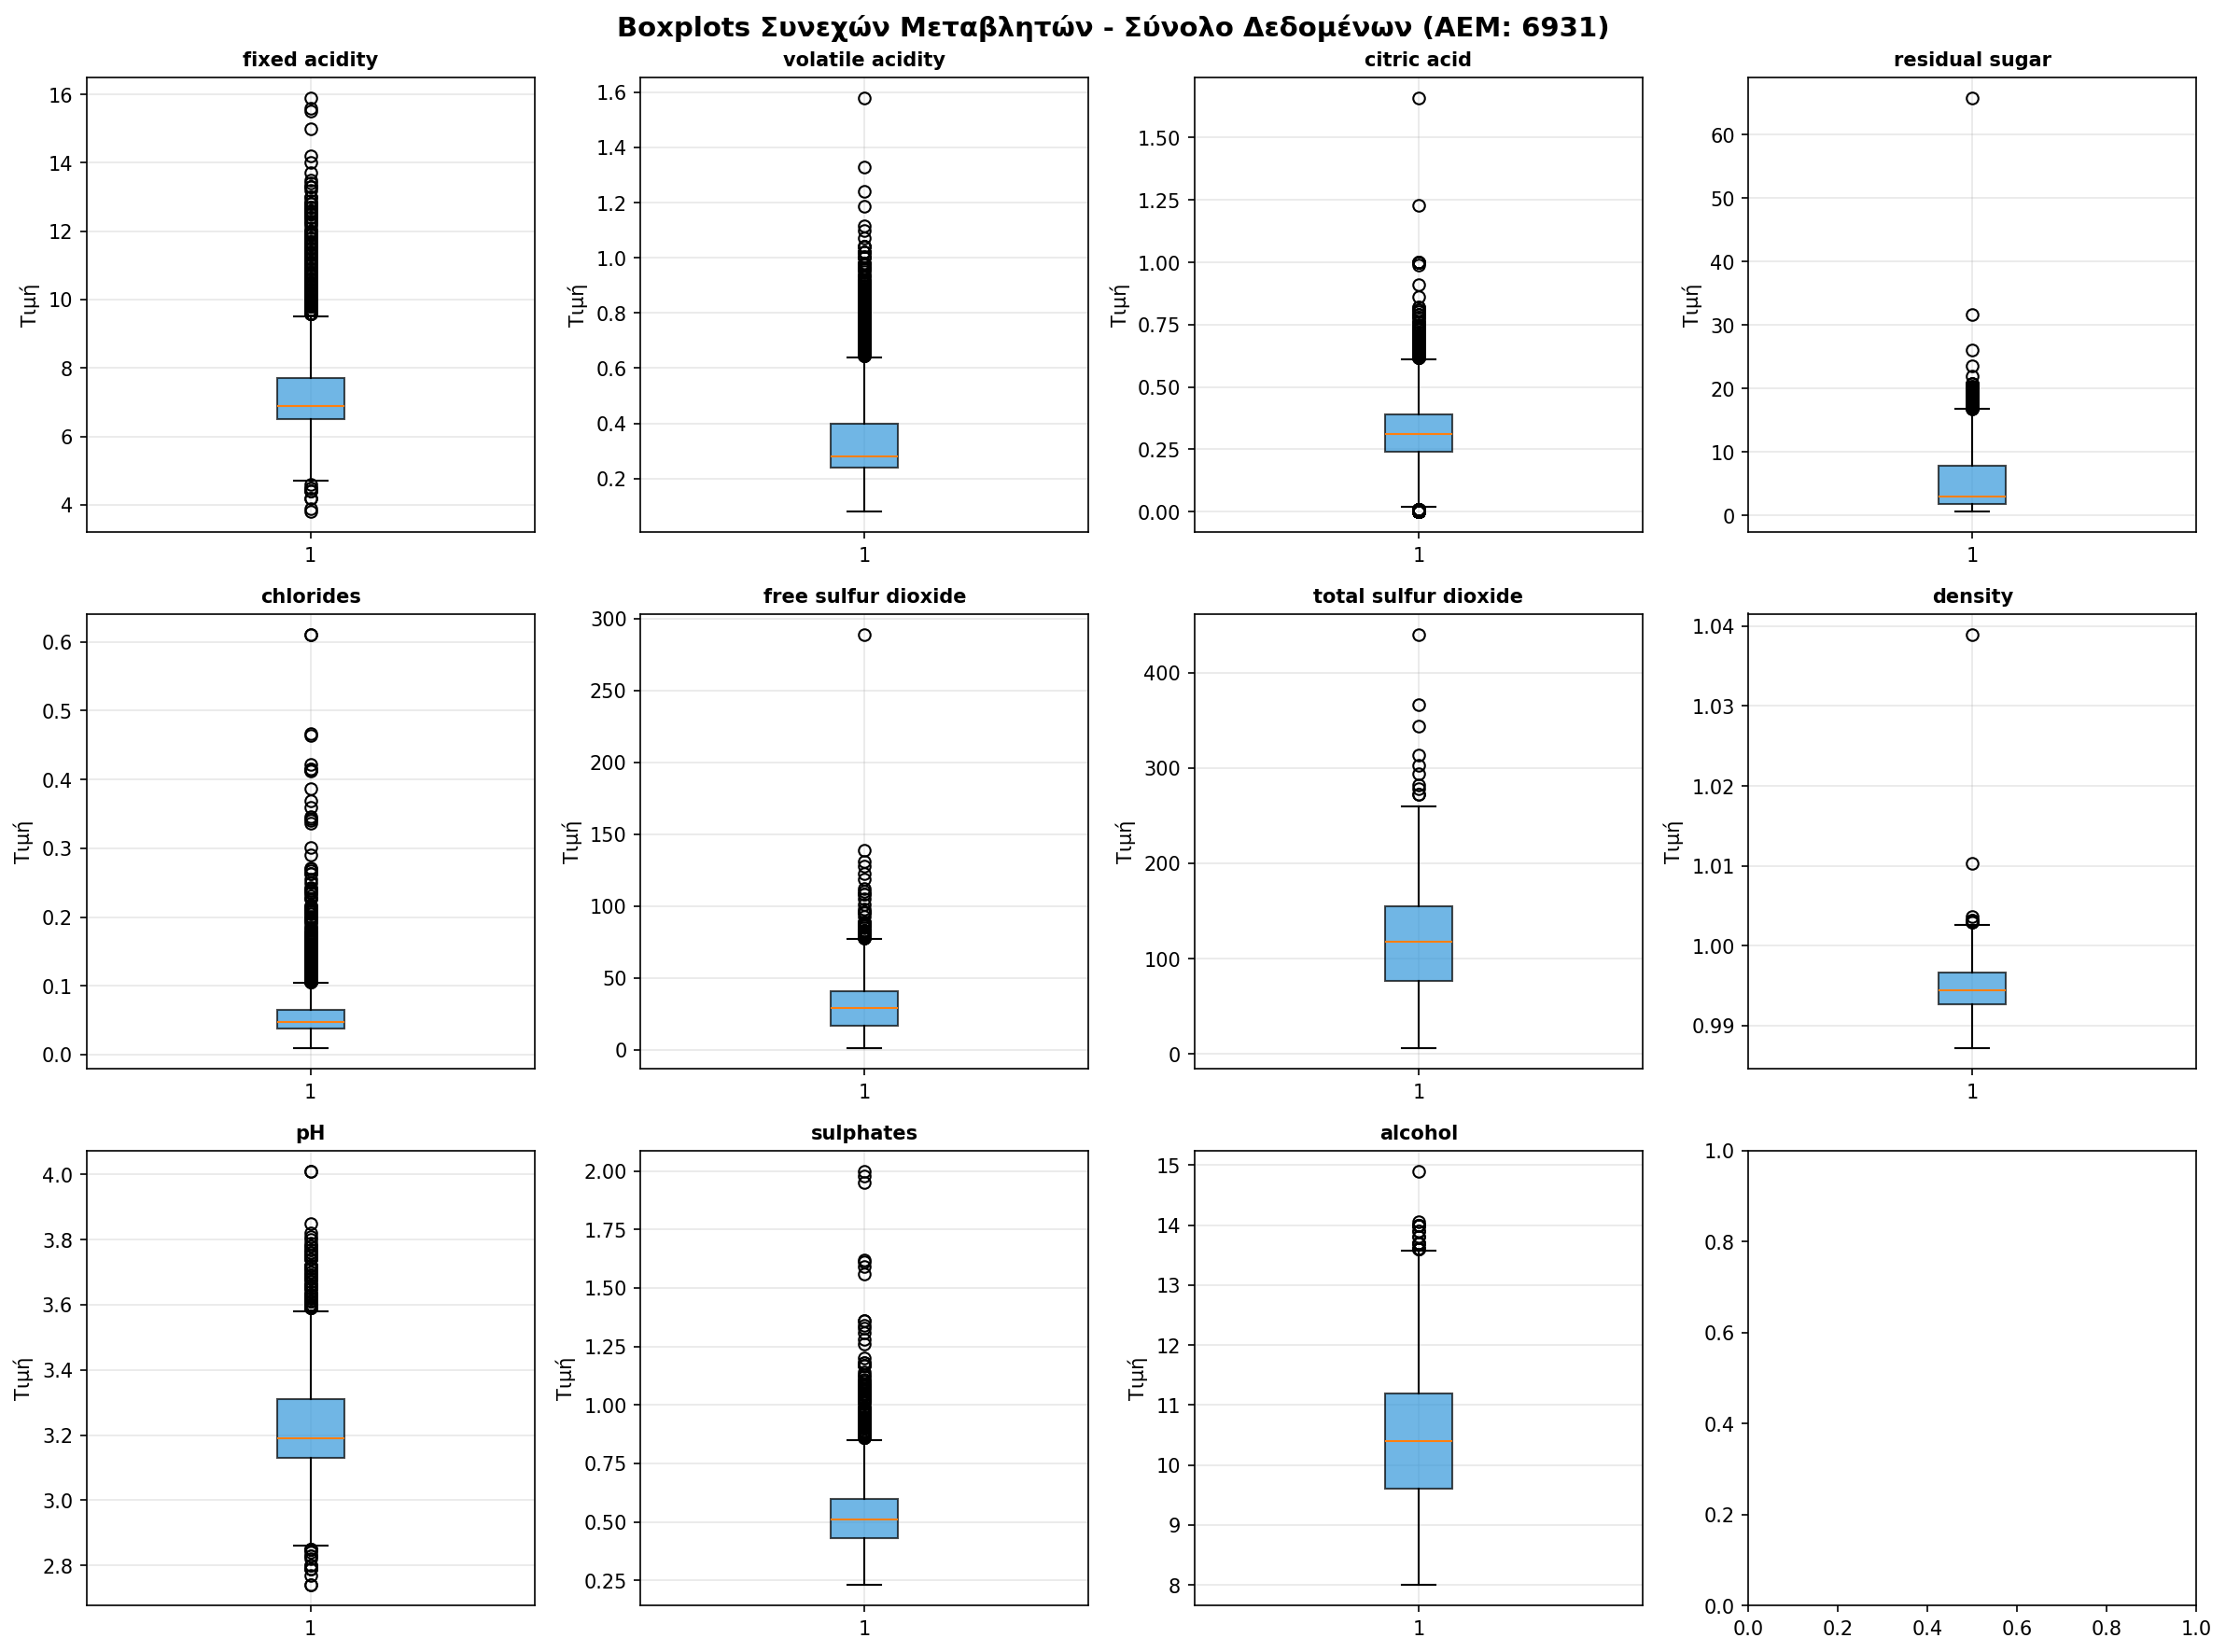
\includegraphics[width=0.95\textwidth]{boxplots_all_data.png}
\caption{Boxplots όλων των συνεχών μεταβλητών για το σύνολο του dataset}
\end{figure}

\textbf{Σχολιασμός:}

\begin{itemize}
    \item \textbf{Fixed acidity:} Σχετικά συμμετρική κατανομή με κέντρο περίπου στο 7. Υπάρχουν μερικά outliers στις υψηλές τιμές.
    
    \item \textbf{Volatile acidity:} Θετικά ασύμμετρη κατανομή (η διάμεσος είναι χαμηλά στο κουτί). Πολλά outliers στις υψηλές τιμές, υποδεικνύοντας ότι λίγα κρασιά έχουν πολύ υψηλή πτητική οξύτητα.
    
    \item \textbf{Citric acid:} Διάμεσος κοντά στο 0.3 με αρκετά outliers. Η κατανομή είναι ελαφρώς θετικά ασύμμετρη.
    
    \item \textbf{Residual sugar:} Πολύ θετικά ασύμμετρη κατανομή με πολλά outliers. Τα περισσότερα κρασιά έχουν χαμηλά υπολειμματικά σάκχαρα, αλλά υπάρχουν γλυκά κρασιά με πολύ υψηλές τιμές.
    
    \item \textbf{Chlorides:} Πολύ συμπαγής κατανομή (μικρό IQR) με πολλά outliers. Οι περισσότερες τιμές είναι κοντά στο 0.05.
    
    \item \textbf{Free sulfur dioxide:} Θετικά ασύμμετρη με outliers στις υψηλές τιμές.
    
    \item \textbf{Total sulfur dioxide:} Παρόμοια με το free SO2, θετικά ασύμμετρη κατανομή.
    
    \item \textbf{Density:} Πολύ συμμετρική κατανομή με κέντρο κοντά στο 0.995. Λίγα outliers.
    
    \item \textbf{pH:} Σχεδόν τέλεια συμμετρική κατανομή (κανονική). Διάμεσος περίπου 3.2.
    
    \item \textbf{Sulphates:} Ελαφρώς θετικά ασύμμετρη με outliers στις υψηλές τιμές.
    
    \item \textbf{Alcohol:} Σχετικά συμμετρική κατανομή με εύρος 8-14\%.
\end{itemize}

\subsection{Κατανομή Quality (Διακριτή Μεταβλητή)}

Η μεταβλητή \textbf{quality} είναι διακριτή (παίρνει ακέραιες τιμές 3-9) και δεν ταιριάζει καλά σε ένα κλασικό boxplot. Γι' αυτό παρουσιάζουμε την κατανομή της με ιστόγραμμα:

\begin{figure}[H]
\centering
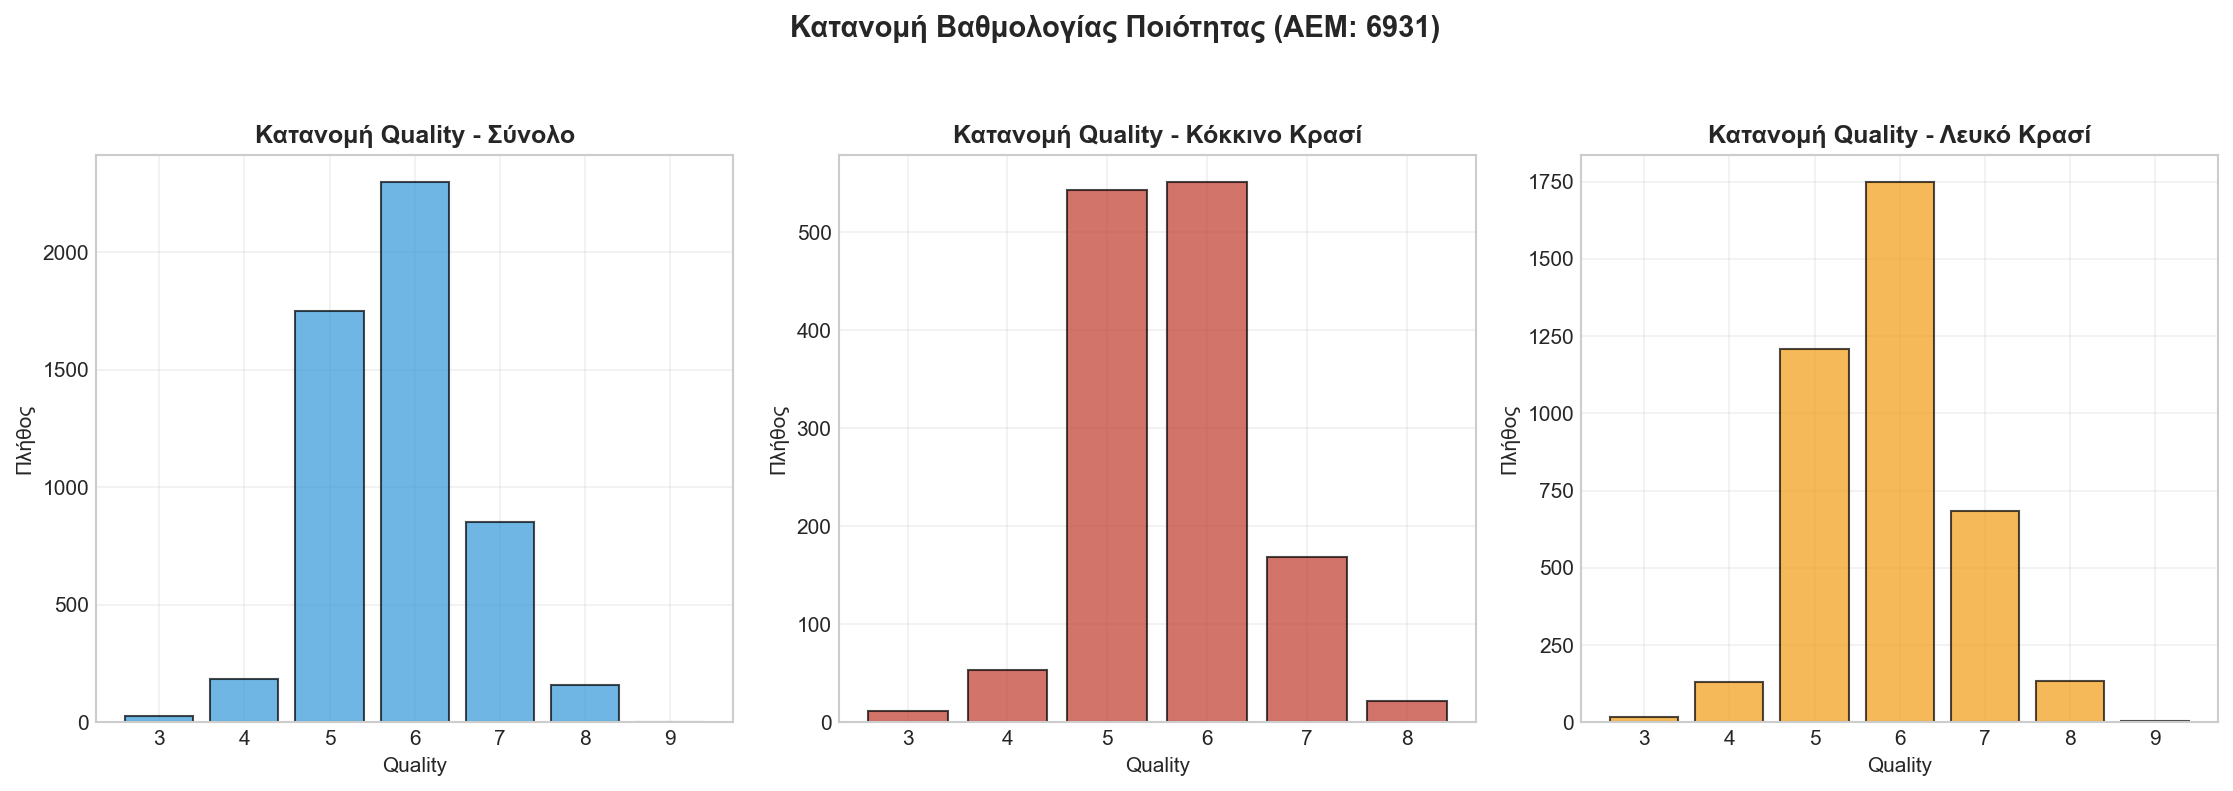
\includegraphics[width=0.95\textwidth]{quality_distribution.png}
\caption{Κατανομή της Quality - Συνολικά και ανά τύπο κρασιού}
\end{figure}

\textbf{Σχολιασμός:}

\begin{itemize}
    \item Η συνολική κατανομή της quality είναι \textbf{κανονική προς τα αριστερά}, με τη μεγαλύτερη συχνότητα στο score 6 (2.299 κρασιά)
    \item \textbf{Κόκκινα κρασιά:} Περισσότερα κρασιά με χαμηλές βαθμολογίες (5-6), με λίγα εξαιρετικά κρασιά (8-9)
    \item \textbf{Λευκά κρασιά:} Πιο ευρεία κατανομή με αρκετά κρασιά στις μεσαίες βαθμολογίες (5-7)
    \item Η μεσοελάχιστη κατανομή υποδεικνύει ότι είναι δύσκολο να παράξεις κρασί με πολύ υψηλή ή πολύ χαμηλή ποιότητα
\end{itemize}

\subsection{Boxplots ανά Τύπο Κρασιού}

\begin{lstlisting}
# Boxplots by wine type
fig, axes = plt.subplots(3, 4, figsize=(16, 12))
for i, col in enumerate(continuous_vars):
    ax = axes[i//4, i%4]
    df.boxplot(column=col, by='wine_type', ax=ax)
    ax.set_title(col)
    ax.set_xlabel('')
plt.suptitle('Boxplots by Wine Type', y=1.02)
plt.tight_layout()
plt.savefig('boxplots_by_wine_type.png')
\end{lstlisting}

\begin{figure}[H]
\centering
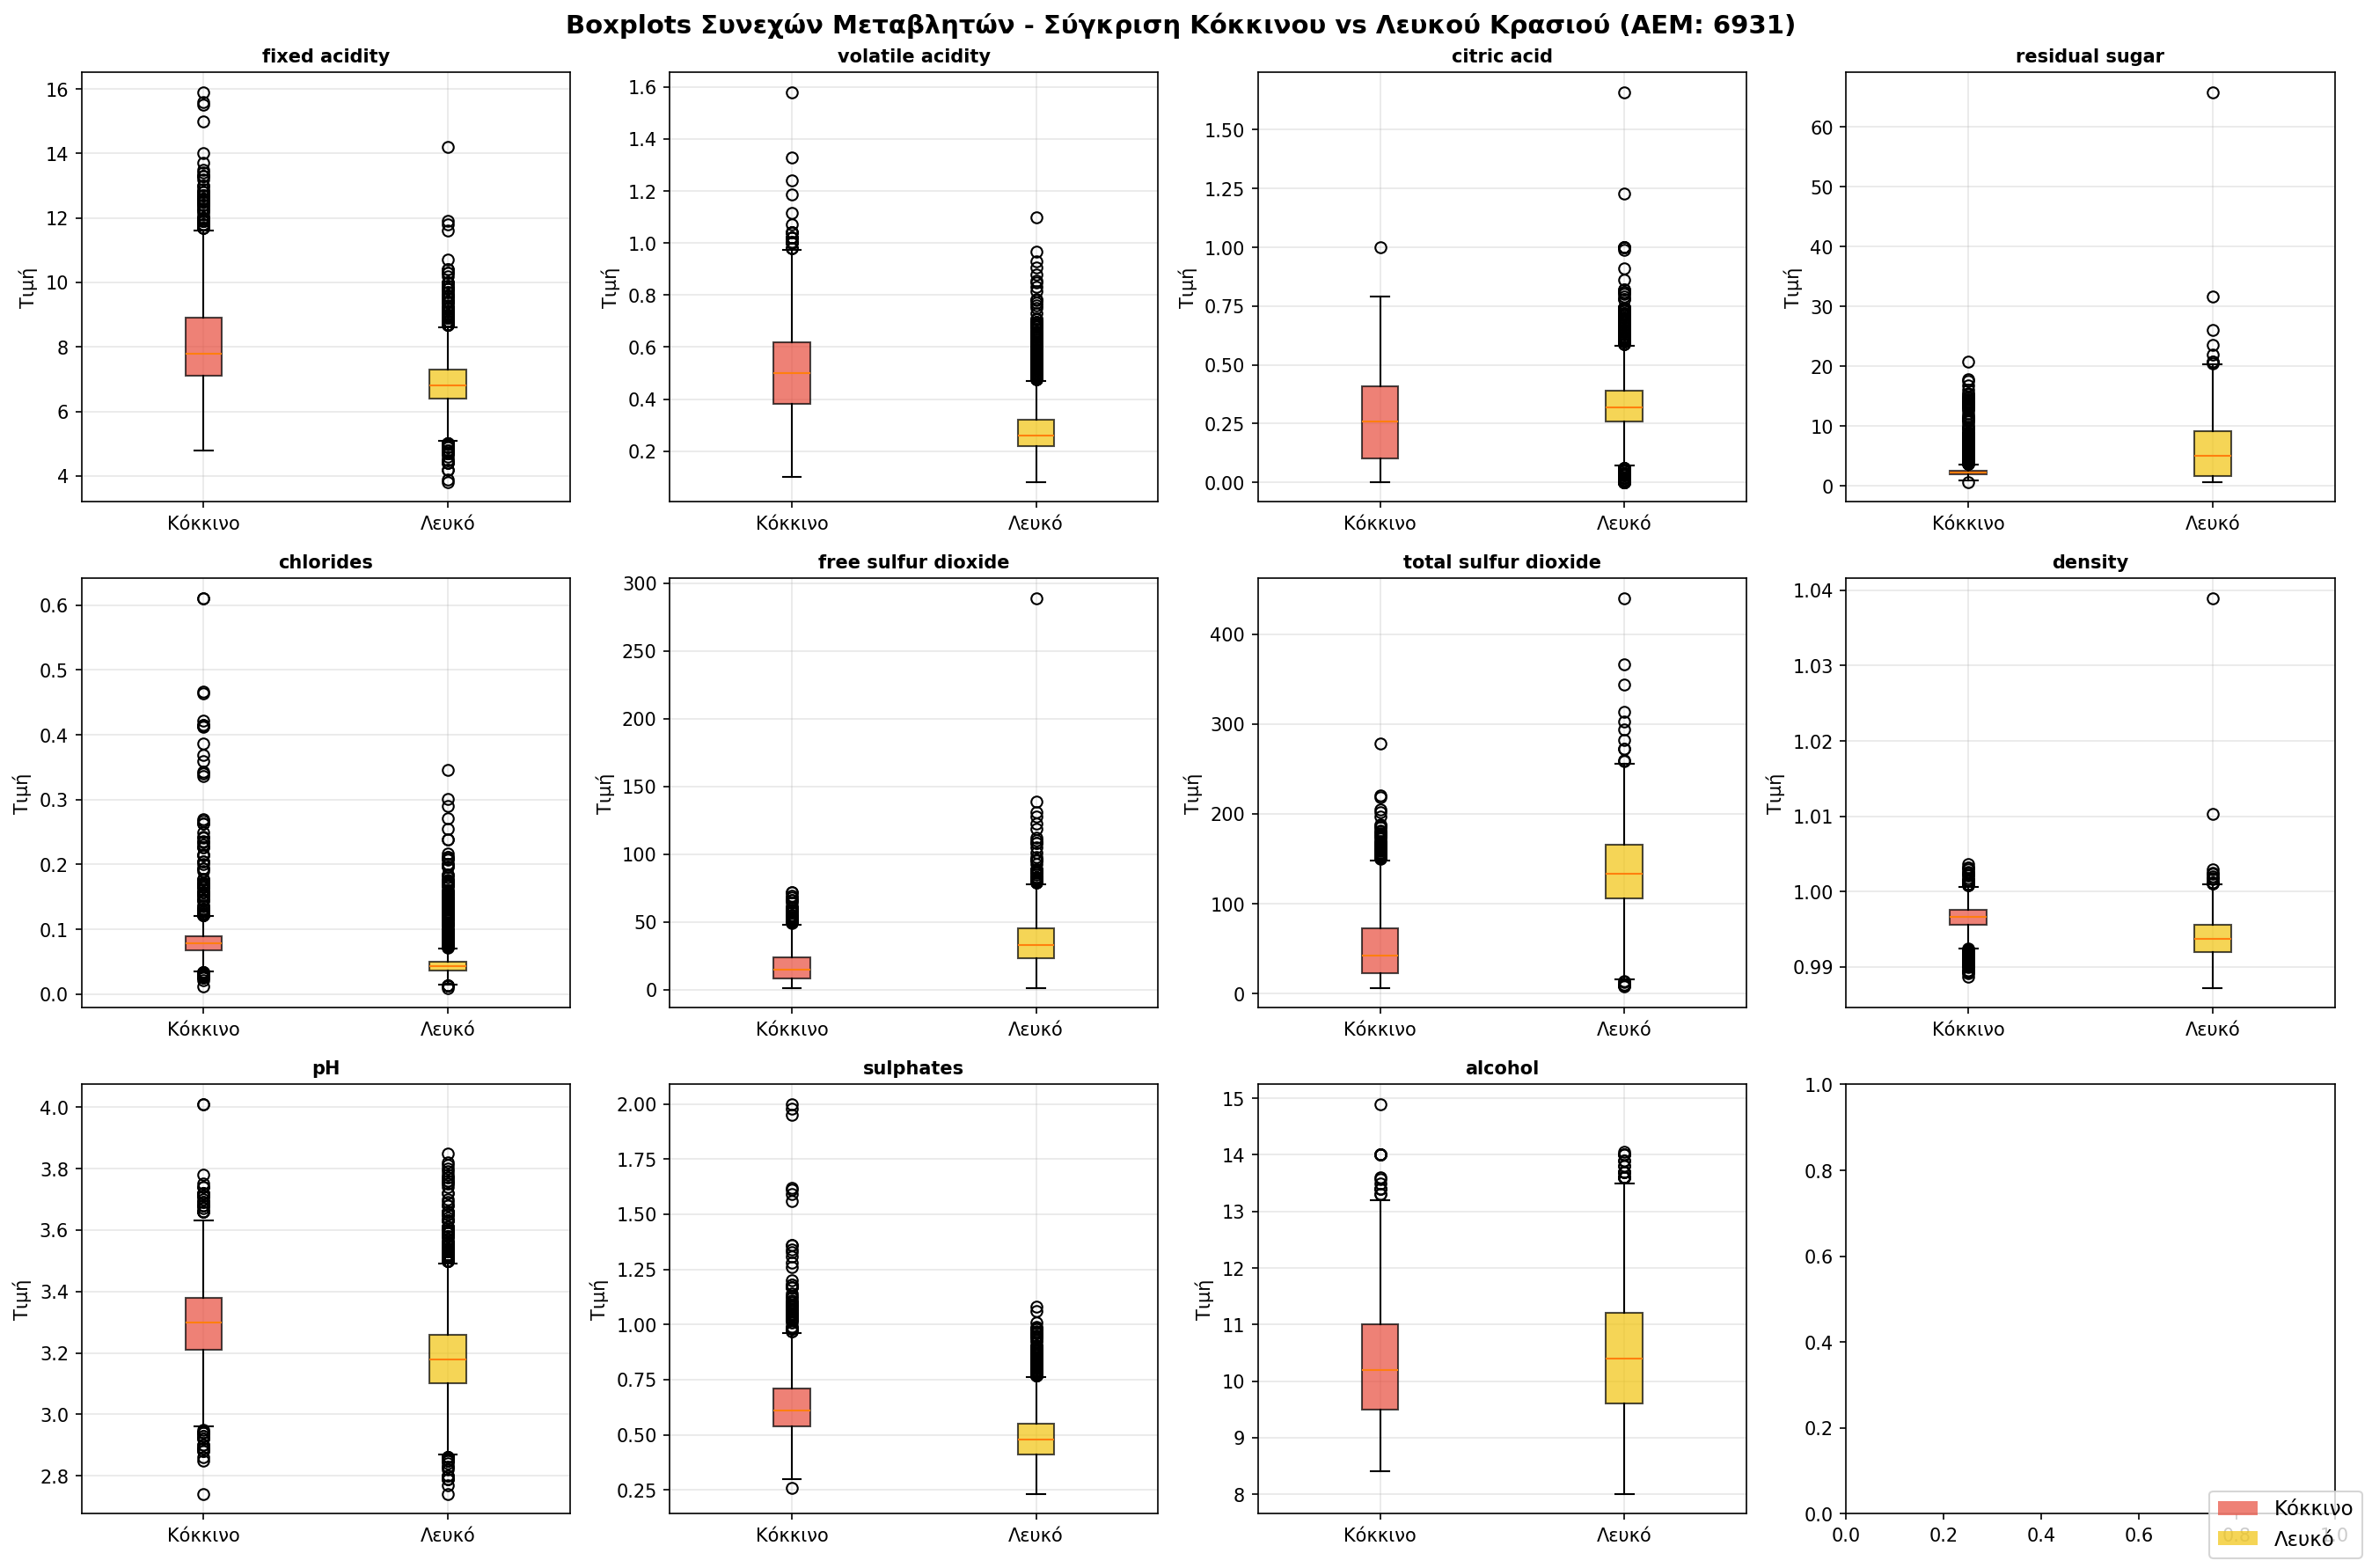
\includegraphics[width=0.95\textwidth]{boxplots_by_wine_type.png}
\caption{Boxplots όλων των συνεχών μεταβλητών ξεχωριστά για κόκκινο και λευκό κρασί}
\end{figure}

\textbf{Σχολιασμός - Διαφορές μεταξύ κόκκινου και λευκού κρασιού:}

\begin{enumerate}
    \item \textbf{Fixed acidity:}
    \begin{itemize}
        \item Κόκκινο: Υψηλότερη διάμεσος (~7.8) και μεγαλύτερη διασπορά
        \item Λευκό: Χαμηλότερη διάμεσος (~6.8) και πιο συμπαγής κατανομή
        \item \textit{Ερμηνεία:} Τα κόκκινα κρασιά τείνουν να έχουν υψηλότερη σταθερή οξύτητα
    \end{itemize}
    
    \item \textbf{Volatile acidity:}
    \begin{itemize}
        \item Κόκκινο: Σημαντικά υψηλότερη (διάμεσος ~0.5)
        \item Λευκό: Πολύ χαμηλότερη (διάμεσος ~0.26)
        \item Το κουτί των κόκκινων είναι μεγαλύτερο, άρα μεγαλύτερη διασπορά (IQR) στην πτητική οξύτητα
        \item \textit{Ερμηνεία:} Η πτητική οξύτητα σχετίζεται με οξικό οξύ - τα λευκά κρασιά είναι πιο ``καθαρά''
    \end{itemize}
    
    \item \textbf{Citric acid:}
    \begin{itemize}
        \item Κόκκινο: Διάμεσος ~0.25
        \item Λευκό: Διάμεσος ~0.32
        \item Παρόμοιες κατανομές με μικρές διαφορές
    \end{itemize}
    
    \item \textbf{Residual sugar:}
    \begin{itemize}
        \item Κόκκινο: Πολύ χαμηλά επίπεδα (διάμεσος ~2.2), τα περισσότερα είναι ``dry''
        \item Λευκό: Υψηλότερα επίπεδα (διάμεσος ~5), μεγαλύτερη ποικιλία (dry έως sweet)
        \item Στα λευκά το κουτί είναι σαφώς μεγαλύτερο, δείχνοντας πολύ μεγαλύτερη διασπορά στα υπολειμματικά σάκχαρα
        \item \textit{Ερμηνεία:} Τα λευκά κρασιά συχνά είναι πιο γλυκά
    \end{itemize}
    
    \item \textbf{Chlorides:}
    \begin{itemize}
        \item Κόκκινο: Υψηλότερα (~0.078)
        \item Λευκό: Χαμηλότερα (~0.043)
        \item Το κουτί είναι σχετικά μικρό και στους δύο τύπους, άρα η κύρια μάζα τιμών είναι συγκεντρωμένη κοντά στη διάμεσο
    \end{itemize}
    
    \item \textbf{Free \& Total sulfur dioxide:}
    \begin{itemize}
        \item Κόκκινο: Πολύ χαμηλά επίπεδα (total SO2 διάμεσος ~42, free SO2 ~15)
        \item Λευκό: Πολύ υψηλότερα επίπεδα (total SO2 διάμεσος ~133, free SO2 ~33)
        \item Για το total SO2, το κουτί των λευκών είναι μεγαλύτερο, άρα και μεγαλύτερη διασπορά στη μεσαία περιοχή τιμών
        \item \textit{Ερμηνεία:} Τα λευκά κρασιά χρειάζονται περισσότερο SO2 ως συντηρητικό επειδή είναι πιο ευαίσθητα στην οξείδωση
    \end{itemize}
    
    \item \textbf{Density:}
    \begin{itemize}
        \item Κόκκινο: Διάμεσος ~0.997
        \item Λευκό: Διάμεσος ~0.994
        \item Ελαφρώς υψηλότερη πυκνότητα στα κόκκινα λόγω υψηλότερων σακχάρων και εκχυλισμάτων
    \end{itemize}
    
    \item \textbf{pH:}
    \begin{itemize}
        \item Κόκκινο: Διάμεσος ~3.30
        \item Λευκό: Διάμεσος ~3.18
        \item Τα λευκά είναι ελαφρώς πιο όξινα
    \end{itemize}
    
    \item \textbf{Sulphates:}
    \begin{itemize}
        \item Κόκκινο: Υψηλότερα (~0.61)
        \item Λευκό: Χαμηλότερα (~0.48)
    \end{itemize}
    
    \item \textbf{Alcohol:}
    \begin{itemize}
        \item Παρόμοια κατανομή και για τους δύο τύπους
        \item Διάμεσος περίπου 10-10.5\% και για τα δύο
        \item Παρόμοιο μέγεθος κουτιού, άρα παρόμοια διασπορά (IQR) στο αλκοόλ
    \end{itemize}
    
    \item \textbf{Quality:}
    \begin{itemize}
        \item Παρόμοια κατανομή με διάμεσο 6 και για τα δύο
        \item Τα λευκά έχουν ελαφρώς μεγαλύτερο εύρος βαθμολογιών
        \item Το σχετικά μικρό κουτί και στους δύο τύπους δείχνει ότι οι περισσότερες τιμές συγκεντρώνονται γύρω από 5-6
    \end{itemize}
\end{enumerate}

\subsection{Συμπεράσματα Ερωτήματος 2}

Από την ανάλυση των boxplots προκύπτουν τα εξής βασικά συμπεράσματα:

\begin{enumerate}
    \item \textbf{Οι περισσότερες μεταβλητές έχουν outliers}, ιδιαίτερα οι residual sugar, chlorides, και sulfur dioxide.
    
    \item \textbf{Πολλές κατανομές είναι θετικά ασύμμετρες} (ουρά προς τα δεξιά), κάτι που είναι συνηθισμένο σε χημικές μετρήσεις.
    
    \item \textbf{Τα κόκκινα και λευκά κρασιά διαφέρουν σημαντικά} σε πολλές μεταβλητές:
    \begin{itemize}
        \item Τα κόκκινα έχουν υψηλότερη πτητική οξύτητα και θειικά άλατα
        \item Τα λευκά έχουν υψηλότερα επίπεδα SO2 και υπολειμματικών σακχάρων
    \end{itemize}
    
    \item \textbf{Τα boxplots αποκαλύπτουν outliers} που μπορεί να επηρεάσουν τις αναλύσεις και πρέπει να αντιμετωπιστούν (βλ. Ερώτημα 3).
    
    \item \textbf{Η διαχωρισμός ανά τύπο κρασιού είναι απαραίτητος} για σωστή ερμηνεία, καθώς οι δύο τύποι έχουν διαφορετικά χημικά χαρακτηριστικά.
\end{enumerate}

%=============================================================================
% ΕΡΩΤΗΜΑ 3: ΑΚΡΑΙΕΣ ΤΙΜΕΣ (OUTLIERS)
%=============================================================================
\newpage
\section{Ερώτημα 3: Εντοπισμός και Μετασχηματισμός Ακραίων Τιμών}

\subsection{Τι είναι οι Ακραίες Τιμές (Outliers);}

Οι \textbf{ακραίες τιμές} (outliers) είναι παρατηρήσεις που απέχουν σημαντικά από τις υπόλοιπες τιμές ενός δείγματος. Μπορεί να οφείλονται σε:

\begin{itemize}
    \item \textbf{Σφάλματα μέτρησης} ή καταχώρησης
    \item \textbf{Πραγματικές ακραίες τιμές} (π.χ. ένα εξαιρετικά γλυκό κρασί)
    \item \textbf{Φυσική ποικιλομορφία} στα δεδομένα
\end{itemize}

Οι outliers μπορούν να παραμορφώσουν τα αποτελέσματα μιας στατιστικής ανάλυσης (π.χ. τον μέσο όρο, τη διασπορά, τη συσχέτιση), γι' αυτό πρέπει να εντοπίζονται και να αντιμετωπίζονται κατάλληλα.

\subsection{Μέθοδος IQR (Interquartile Range)}

\subsubsection{Πώς λειτουργεί η μέθοδος IQR}

Η μέθοδος IQR χρησιμοποιεί τα τεταρτημόρια (quartiles) για να ορίσει τα όρια εκτός των οποίων μια τιμή θεωρείται ακραία. Υπολογίζεται ως εξής:

\textbf{Βήμα 1:} Υπολογισμός τεταρτημορίων
\begin{itemize}
    \item $Q1$ = 25ο εκατοστημόριο (το 25\% των τιμών είναι μικρότερες)
    \item $Q3$ = 75ο εκατοστημόριο (το 75\% των τιμών είναι μικρότερες)
\end{itemize}

\textbf{Βήμα 2:} Υπολογισμός IQR
$$\text{IQR} = Q3 - Q1$$

\textbf{Βήμα 3:} Υπολογισμός ορίων
$$\text{Κάτω όριο} = Q1 - 1.5 \times \text{IQR}$$
$$\text{Άνω όριο} = Q3 + 1.5 \times \text{IQR}$$

\textbf{Βήμα 4:} Κάθε τιμή $x$ που ικανοποιεί $x < \text{Κάτω όριο}$ ή $x > \text{Άνω όριο}$ θεωρείται \textbf{outlier}.

\subsubsection{Παράδειγμα}

Έστω ότι έχουμε τιμές pH: $Q1 = 3.13$, $Q3 = 3.31$.

$$\text{IQR} = 3.31 - 3.13 = 0.18$$
$$\text{Κάτω όριο} = 3.13 - 1.5 \times 0.18 = 2.86$$
$$\text{Άνω όριο} = 3.31 + 1.5 \times 0.18 = 3.58$$

Κάθε κρασί με pH $< 2.86$ ή pH $> 3.58$ θεωρείται outlier.

\subsubsection{Πλεονεκτήματα μεθόδου IQR}

\begin{itemize}
    \item Δεν επηρεάζεται από ακραίες τιμές (βασίζεται σε τεταρτημόρια, όχι μέσο όρο)
    \item Δεν απαιτεί κανονική κατανομή
    \item Εύκολη στην κατανόηση και εφαρμογή
\end{itemize}

\subsubsection{Κώδικας IQR στην Python}

\begin{lstlisting}
for var in continuous_vars:
    Q1 = df[var].quantile(0.25)
    Q3 = df[var].quantile(0.75)
    IQR = Q3 - Q1

    lower_bound = Q1 - 1.5 * IQR
    upper_bound = Q3 + 1.5 * IQR

    outliers = (df[var] < lower_bound) | (df[var] > upper_bound)
    print(f"{var}: {outliers.sum()} outliers")
\end{lstlisting}

\subsubsection{Αποτελέσματα μεθόδου IQR}

\begin{itemize}
    \item Fixed acidity: 270 outliers (5.1\%)
    \item Volatile acidity: 308 outliers (5.8\%)
    \item Citric acid: 327 outliers (6.2\%)
    \item Residual sugar: 124 outliers (2.4\%)
    \item Chlorides: 232 outliers (4.4\%)
    \item Free sulfur dioxide: 48 outliers (0.9\%)
    \item Total sulfur dioxide: 10 outliers (0.2\%)
    \item Density: 7 outliers (0.1\%)
    \item pH: 104 outliers (2.0\%)
    \item Sulphates: 146 outliers (2.8\%)
    \item Alcohol: 29 outliers (0.5\%)
    \item Quality: 188 outliers (3.6\%)
\end{itemize}

\textbf{Σύνολο ακραίων τιμών (IQR): 1.793}

\subsection{Μέθοδος Z-Score}

\subsubsection{Πώς λειτουργεί η μέθοδος Z-Score}

Η μέθοδος Z-Score μετράει πόσες \textbf{τυπικές αποκλίσεις} ($\sigma$) απέχει κάθε τιμή από τον \textbf{μέσο όρο} ($\mu$) της μεταβλητής.

\paragraph{Τι είναι η Τυπική Απόκλιση;}

Η \textbf{τυπική απόκλιση} (standard deviation, $\sigma$) είναι ένα μέτρο που μας δείχνει \textbf{πόσο διασκορπισμένες είναι οι τιμές γύρω από τον μέσο όρο}. Με άλλα λόγια:

\begin{itemize}
    \item Αν η τυπική απόκλιση είναι \textbf{μικρή}, οι τιμές είναι \textbf{κοντά στον μέσο όρο} (δεν υπάρχει μεγάλη διασπορά)
    \item Αν η τυπική απόκλιση είναι \textbf{μεγάλη}, οι τιμές είναι \textbf{απλωμένες πολύ} (υπάρχει μεγάλη διασπορά)
\end{itemize}

Υπολογίζεται με τη εξίσωση:
$$\sigma = \sqrt{\frac{1}{n} \sum_{i=1}^{n} (x_i - \mu)^2}$$

δηλαδή, η τετραγωνική ρίζα του μέσου όρου των τετραγώνων των αποκλίσεων από τον μέσο όρο.

\textbf{Στα δεδομένα μας (κρασιά):}

Για τη μεταβλητή alcohol:
\begin{itemize}
    \item Μέσος όρος ($\mu$) = 10.49\%
    \item Τυπική απόκλιση ($\sigma$) = 1.11\%
\end{itemize}

Αυτό σημαίνει ότι οι περισσότερες τιμές κυμαίνονται περίπου μεταξύ $10.49 - 1.11 = 9.38$\% και $10.49 + 1.11 = 11.60$\%.

\textbf{Βήμα 1:} Υπολογισμός Z-Score κάθε τιμής
$$z = \frac{x - \mu}{\sigma}$$

όπου:
\begin{itemize}
    \item $x$ = η τιμή που εξετάζουμε
    \item $\mu$ = ο μέσος όρος της μεταβλητής
    \item $\sigma$ = η τυπική απόκλιση της μεταβλητής
\end{itemize}

Το Z-Score μας λέει πόσες τυπικές αποκλίσεις απέχει μια τιμή από τον μέσο.

\textbf{Βήμα 2:} Αν $|z| > 3.5$ (δηλαδή η τιμή απέχει πάνω από 3.5 τυπικές αποκλίσεις), θεωρείται \textbf{outlier}.

Αυτά τα όρια μεταφράζονται σε:
$$\text{Κάτω όριο} = \mu - 3.5 \times \sigma$$
$$\text{Άνω όριο} = \mu + 3.5 \times \sigma$$

\subsubsection{Παράδειγμα}

Για τη μεταβλητή alcohol, αν $\mu = 10.49$ και $\sigma = 1.11$:

$$\text{Κάτω όριο} = 10.49 - 3.5 \times 1.11 = 6.60$$
$$\text{Άνω όριο} = 10.49 + 3.5 \times 1.11 = 14.38$$

Ένα κρασί με alcohol = 15\% θα θεωρηθεί outlier αφού $15 > 14.38$.

\subsubsection{Πλεονεκτήματα και μειονεκτήματα μεθόδου Z-Score}

\textbf{Πλεονεκτήματα:}
\begin{itemize}
    \item Βασίζεται σε μαθηματικά σαφή κριτήρια
    \item Ρυθμιζόμενο threshold (στην περίπτωσή μας 3.5)
\end{itemize}

\textbf{Μειονεκτήματα:}
\begin{itemize}
    \item Ο μέσος όρος και η τυπική απόκλιση επηρεάζονται από τις ίδιες τις ακραίες τιμές
    \item Υποθέτει (ιδανικά) κανονική ή σχεδόν κανονική κατανομή
\end{itemize}

\subsubsection{Κώδικας Z-Score στην Python}

\begin{lstlisting}
z_threshold = 3.5
for var in continuous_vars:
    mean = df[var].mean()
    std = df[var].std()

    lower_bound = mean - z_threshold * std
    upper_bound = mean + z_threshold * std

    outliers = (df[var] < lower_bound) | (df[var] > upper_bound)
    print(f"{var}: {outliers.sum()} outliers")
\end{lstlisting}

\subsubsection{Αποτελέσματα μεθόδου Z-Score ($|z| > 3.5$)}

\begin{itemize}
    \item Fixed acidity: 76 outliers (1.4\%)
    \item Volatile acidity: 39 outliers (0.7\%)
    \item Citric acid: 12 outliers (0.2\%)
    \item Residual sugar: 5 outliers (0.1\%)
    \item Chlorides: 56 outliers (1.1\%)
    \item Free sulfur dioxide: 18 outliers (0.3\%)
    \item Total sulfur dioxide: 4 outliers (0.1\%)
    \item Density: 2 outliers (0.04\%)
    \item pH: 16 outliers (0.3\%)
    \item Sulphates: 39 outliers (0.7\%)
    \item Alcohol: 1 outlier (0.02\%)
    \item Quality: 3 outliers (0.1\%)
\end{itemize}

\textbf{Σύνολο ακραίων τιμών (Z-Score): 271}

\subsection{Σύγκριση Μεθόδων IQR vs Z-Score}

\begin{itemize}
    \item Η μέθοδος \textbf{IQR εντοπίζει 1.793 outliers} ενώ η μέθοδος \textbf{Z-Score εντοπίζει 271}
    \item Η IQR είναι πιο \textbf{ευαίσθητη} (αυστηρότερη) -- εντοπίζει περισσότερες ακραίες τιμές
    \item Η Z-Score με threshold 3.5 είναι πιο \textbf{συντηρητική} -- εντοπίζει μόνο τις πολύ ακραίες τιμές
    \item Η διαφορά οφείλεται στο ότι:
    \begin{itemize}
        \item Η IQR ορίζει τα όρια βάσει τεταρτημορίων (1.5 $\times$ IQR)
        \item Η Z-Score ορίζει τα όρια βάσει τυπικών αποκλίσεων (3.5 $\times$ $\sigma$)
        \item Σε ασύμμετρες κατανομές (όπως πολλές μεταβλητές κρασιού), τα όρια IQR γίνονται στενότερα
    \end{itemize}
    \item Στην πράξη, η επιλογή μεθόδου εξαρτάται από το context: αν θέλουμε να είμαστε αυστηροί, χρησιμοποιούμε IQR· αν θέλουμε μόνο τα πιο ακραία σημεία, Z-Score
\end{itemize}

\subsection{Clamp Transformation (Μετασχηματισμός Αποκοπής)}

\subsubsection{Τι είναι το Clamp Transformation;}

Το \textbf{Clamp Transformation} (ή Winsorization) είναι μια τεχνική αντιμετώπισης ακραίων τιμών που \textbf{δεν αφαιρεί} τις παρατηρήσεις, αλλά τις \textbf{αντικαθιστά} με τις πλησιέστερες αποδεκτές τιμές:

\begin{itemize}
    \item Αν $x < \text{Κάτω όριο}$ $\rightarrow$ $x = \text{Κάτω όριο}$
    \item Αν $x > \text{Άνω όριο}$ $\rightarrow$ $x = \text{Άνω όριο}$
    \item Αν η τιμή είναι εντός ορίων $\rightarrow$ παραμένει ως έχει
\end{itemize}

\subsubsection{Γιατί Clamp αντί για αφαίρεση;}

\begin{itemize}
    \item {\textbf{Διατήρηση μεγέθους δείγματος:}} Δεν χάνουμε εγγραφές, πράγμα σημαντικό αν το dataset δεν είναι πολύ μεγάλο
    \item \textbf{Μείωση επίδρασης outliers:} Οι ακραίες τιμές μετριάζονται χωρίς να εξαφανίζονται
    \item \textbf{Διατήρηση δομής:} Δεν αλλάζει η σειρά (ranking) των τιμών
\end{itemize}

\subsubsection{Εφαρμογή: Κώδικας Clamp στην Python}

Εφαρμόζουμε Clamp με βάση τα όρια της μεθόδου IQR:

\begin{lstlisting}
for var in continuous_vars:
    Q1 = df[var].quantile(0.25)
    Q3 = df[var].quantile(0.75)
    IQR = Q3 - Q1
    lower = Q1 - 1.5 * IQR
    upper = Q3 + 1.5 * IQR

    # Clamp: clip values to [lower, upper]
    df[var] = df[var].clip(lower=lower, upper=upper)
\end{lstlisting}

\subsubsection{Αποτελέσματα Clamp Transformation}

Η εφαρμογή του Clamp μετασχηματισμού αφορά \textbf{1.793 τιμές} (βάσει IQR) και μετά τον μετασχηματισμό:

\begin{itemize}
    \item Δεν χάθηκε καμία εγγραφή (παραμένουν 5.274 γραμμές)
    \item Δεν υπάρχουν πλέον outliers βάσει IQR
    \item Οι κατανομές γίνονται πιο συμπαγείς
\end{itemize}

\subsection{Boxplots Πριν και Μετά τον Μετασχηματισμό}

\begin{figure}[H]
\centering
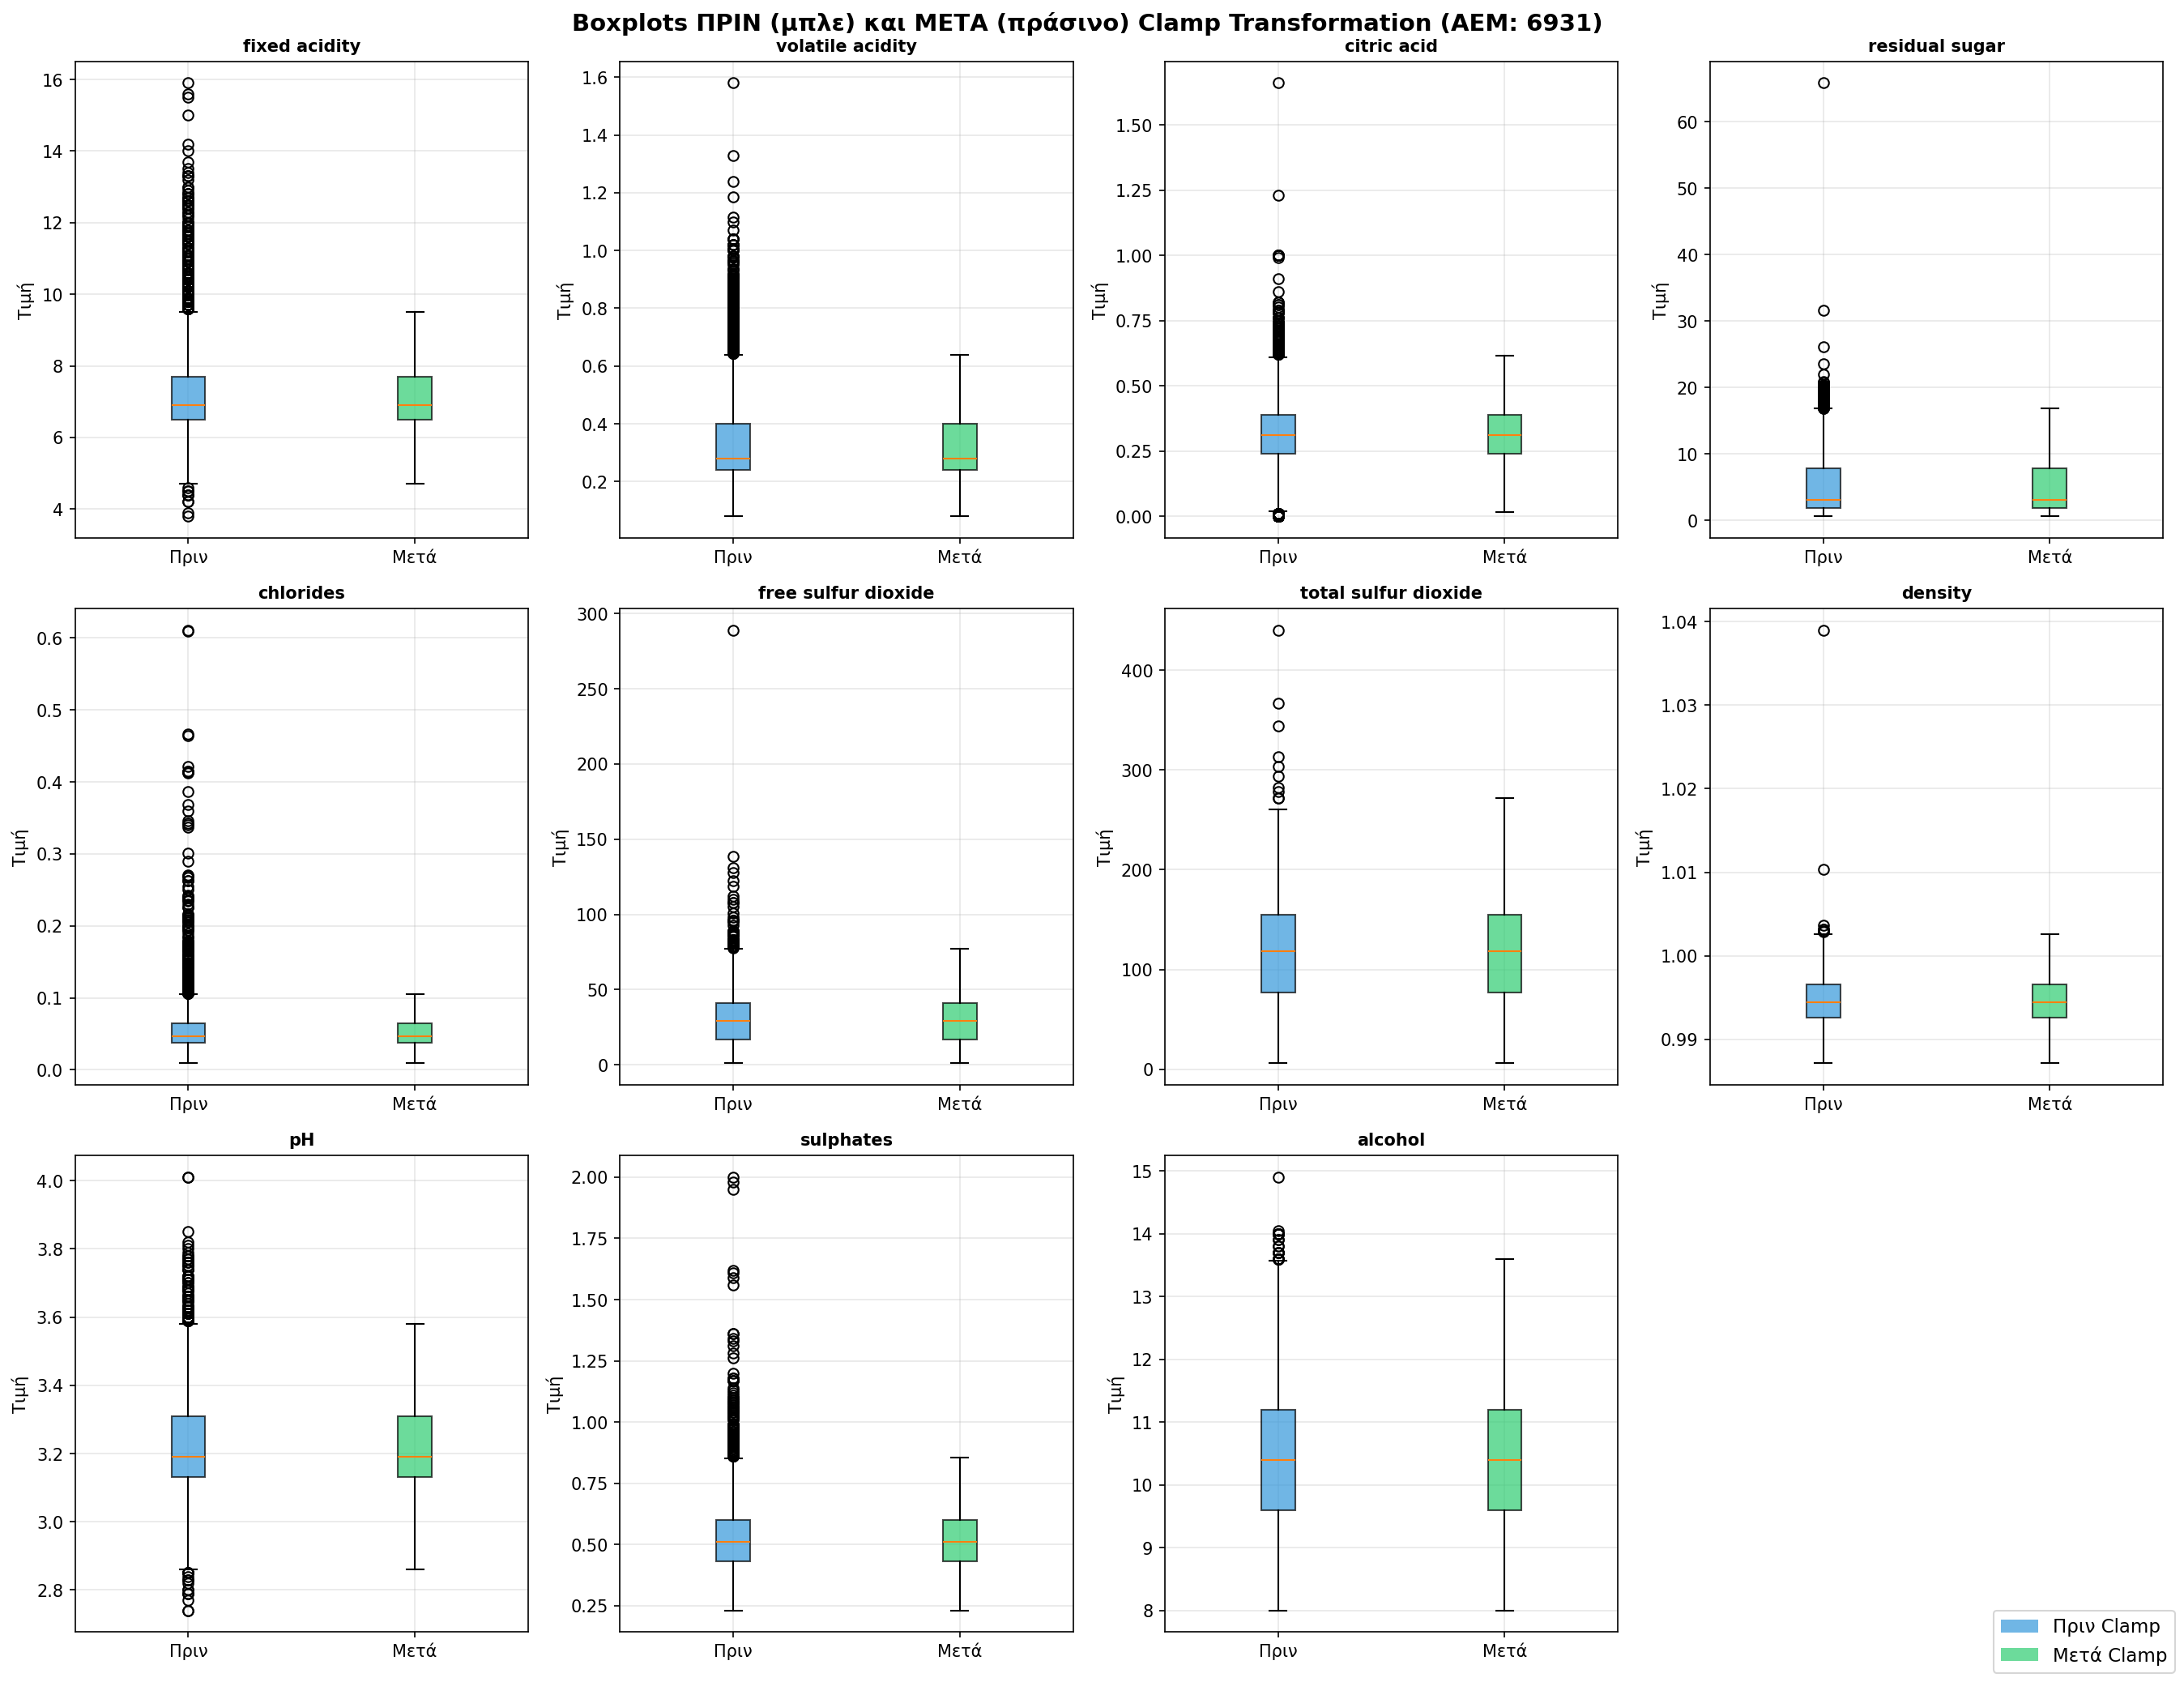
\includegraphics[width=0.95\textwidth]{boxplots_before_after_clamp.png}
\caption{Σύγκριση boxplots πριν (μπλε) και μετά (πράσινο) τον Clamp μετασχηματισμό}
\end{figure}

\textbf{Σχολιασμός:}

\begin{itemize}
    \item Μετά το Clamp, τα μουστάκια τερματίζουν ακριβώς στα όρια IQR
    \item Οι κατανομές γίνονται πιο ομοιόμορφες, χωρίς ακραία σημεία
    \item Οι μεταβλητές με τη μεγαλύτερη αλλαγή (πολλά outliers) είναι: citric acid (327), volatile acidity (308), fixed acidity (270), chlorides (232) και quality (188)
    \item Οι μεταβλητές density (7), total sulfur dioxide (10) και alcohol (29) επηρεάστηκαν ελάχιστα
\end{itemize}

\subsection{Συμπεράσματα Ερωτήματος 3}

\begin{enumerate}
    \item Η μέθοδος \textbf{IQR} εντόπισε 1.793 ακραίες τιμές σε 12 μεταβλητές
    \item Η μέθοδος \textbf{Z-Score} (threshold 3.5) εντόπισε μόλις 271, επιβεβαιώνοντας τον πιο συντηρητικό χαρακτήρα της
    \item Ο \textbf{Clamp μετασχηματισμός} εφαρμόστηκε βάσει IQR, αντικαθιστώντας τις ακραίες τιμές με τα όρια
    \item Το μετασχηματισμένο dataset αποθηκεύτηκε στο αρχείο \texttt{transformed\_wine\_data\_AEM\_6931.csv}
    \item Η επιλογή μεταξύ IQR και Z-Score εξαρτάται από το πλαίσιο: η IQR είναι καταλληλότερη για ασύμμετρες κατανομές, η Z-Score για κανονικές
\end{enumerate}

%=============================================================================
% ΕΡΩΤΗΜΑ 4: ΟΠΤΙΚΗ ΠΑΡΟΥΣΙΑΣΗ ΚΑΙ ΠΕΡΙΓΡΑΦΙΚΑ ΣΤΑΤΙΣΤΙΚΑ
%=============================================================================
\newpage
\section{Ερώτημα 4: Οπτική Παρουσίαση και Περιγραφικά Στατιστικά}

Σε αυτό το ερώτημα παρουσιάζουμε το τελικό ``καθαρό'' σύνολο δεδομένων (μετά τον Clamp μετασχηματισμό) με οπτικοποιήσεις και περιγραφικά στατιστικά.

\subsection{Περιγραφικά Στατιστικά - Συνεχείς Μεταβλητές}

Ο παρακάτω πίνακας παρουσιάζει τα βασικά περιγραφικά στατιστικά για τις 11 συνεχείς μεταβλητές του dataset:

\begin{table}[H]
\centering
\caption{Περιγραφικά Στατιστικά Συνεχών Μεταβλητών (N = 5.274)}
\label{tab:desc_continuous}
\scriptsize
\begin{tabular}{lrrrrrrr}
\toprule
\textbf{Μεταβλητή} & \textbf{N} & \textbf{Missing} & \textbf{Μέση Τιμή} & \textbf{Διάμεσος} & \textbf{Τυπ. Απόκλ.} & \textbf{Min} & \textbf{Max} \\
\midrule
fixed acidity & 5274 & 0 & 7.12 & 6.90 & 1.00 & 4.70 & 9.50 \\
volatile acidity & 5274 & 0 & 0.33 & 0.28 & 0.14 & 0.08 & 0.64 \\
citric acid & 5274 & 0 & 0.31 & 0.31 & 0.13 & 0.02 & 0.62 \\
residual sugar & 5274 & 0 & 5.25 & 3.00 & 4.44 & 0.60 & 16.80 \\
chlorides & 5274 & 0 & 0.053 & 0.047 & 0.021 & 0.009 & 0.106 \\
free sulfur dioxide & 5274 & 0 & 30.20 & 29.00 & 16.76 & 1.00 & 77.00 \\
total sulfur dioxide & 5274 & 0 & 115.52 & 118.00 & 55.75 & 6.00 & 271.81 \\
density & 5274 & 0 & 0.9946 & 0.9944 & 0.0028 & 0.9871 & 1.0026 \\
pH & 5274 & 0 & 3.22 & 3.19 & 0.15 & 2.86 & 3.58 \\
sulphates & 5274 & 0 & 0.53 & 0.51 & 0.13 & 0.23 & 0.86 \\
alcohol & 5274 & 0 & 10.49 & 10.40 & 1.11 & 8.00 & 13.60 \\
\bottomrule
\end{tabular}
\end{table}

\begin{table}[H]
\centering
\caption{Επιπλέον Στατιστικά Συνεχών Μεταβλητών}
\label{tab:desc_continuous2}
\scriptsize
\begin{tabular}{lrrrrrr}
\toprule
\textbf{Μεταβλητή} & \textbf{Q1 (25\%)} & \textbf{Q3 (75\%)} & \textbf{IQR} & \textbf{Εύρος} & \textbf{Ασυμμετρία} & \textbf{Cardinality} \\
\midrule
fixed acidity & 6.50 & 7.70 & 1.20 & 4.80 & 0.63 & 53 \\
volatile acidity & 0.24 & 0.40 & 0.16 & 0.56 & 0.89 & 105 \\
citric acid & 0.24 & 0.39 & 0.15 & 0.60 & -0.05 & 62 \\
residual sugar & 1.80 & 7.80 & 6.00 & 16.20 & 1.10 & 248 \\
chlorides & 0.038 & 0.065 & 0.027 & 0.097 & 0.95 & 95 \\
free sulfur dioxide & 17.00 & 41.00 & 24.00 & 76.00 & 0.51 & 98 \\
total sulfur dioxide & 77.13 & 155.00 & 77.88 & 265.81 & -0.04 & 262 \\
density & 0.9926 & 0.9966 & 0.0040 & 0.0155 & 0.04 & 931 \\
pH & 3.13 & 3.31 & 0.18 & 0.72 & 0.24 & 74 \\
sulphates & 0.43 & 0.60 & 0.17 & 0.63 & 0.63 & 63 \\
alcohol & 9.60 & 11.20 & 1.60 & 5.60 & 0.62 & 95 \\
\bottomrule
\end{tabular}
\end{table}

\textbf{Παρατηρήσεις:}
\begin{itemize}
    \item \textbf{Δεν υπάρχουν missing values} σε καμία μεταβλητή (μετά τον καθαρισμό)
    \item \textbf{Υψηλή ασυμμετρία} (Skewness > 0.5) παρατηρείται στα: residual sugar (1.10), volatile acidity (0.89), chlorides (0.95)
    \item \textbf{Υψηλό cardinality} έχει η density (931 μοναδικές τιμές), ενώ χαμηλό cardinality έχει η fixed acidity (53)
    \item Οι τιμές είναι περιορισμένες στα όρια του Clamp (βλ. min/max)
\end{itemize}

\subsection{Περιγραφικά Στατιστικά - Κατηγορικές Μεταβλητές}

\begin{table}[H]
\centering
\caption{Περιγραφικά Στατιστικά Κατηγορικών Μεταβλητών}
\label{tab:desc_categorical}
\begin{tabular}{lrrllrr}
\toprule
\textbf{Μεταβλητή} & \textbf{N} & \textbf{Missing} & \textbf{Cardinality} & \textbf{Mode} & \textbf{Συχν. Mode} & \textbf{\%} \\
\midrule
wine\_type & 5274 & 0 & 2 & white & 3924 & 74.4\% \\
quality & 5274 & 0 & 7 & 6 & 2299 & 43.6\% \\
\bottomrule
\end{tabular}
\end{table}

\textbf{Κατανομή Wine Type:}
\begin{itemize}
    \item \textbf{Λευκά κρασιά:} 3.924 (74.4\%)
    \item \textbf{Κόκκινα κρασιά:} 1.350 (25.6\%)
\end{itemize}

\textbf{Κατανομή Quality:}
\begin{itemize}
    \item Score 3: 28 (0.5\%)
    \item Score 4: 184 (3.5\%)
    \item Score 5: 1.751 (33.2\%)
    \item Score 6: 2.299 (43.6\%) -- \textit{Πιθανότερη τιμή}
    \item Score 7: 852 (16.2\%)
    \item Score 8: 157 (3.0\%)
    \item Score 9: 3 (0.06\%)
\end{itemize}

\subsection{Boxplots Τελικού Dataset}

Τα boxplots απεικονίζουν την κατανομή κάθε συνεχούς μεταβλητής, ξεχωριστά για κόκκινο και λευκό κρασί:

\begin{figure}[H]
\centering
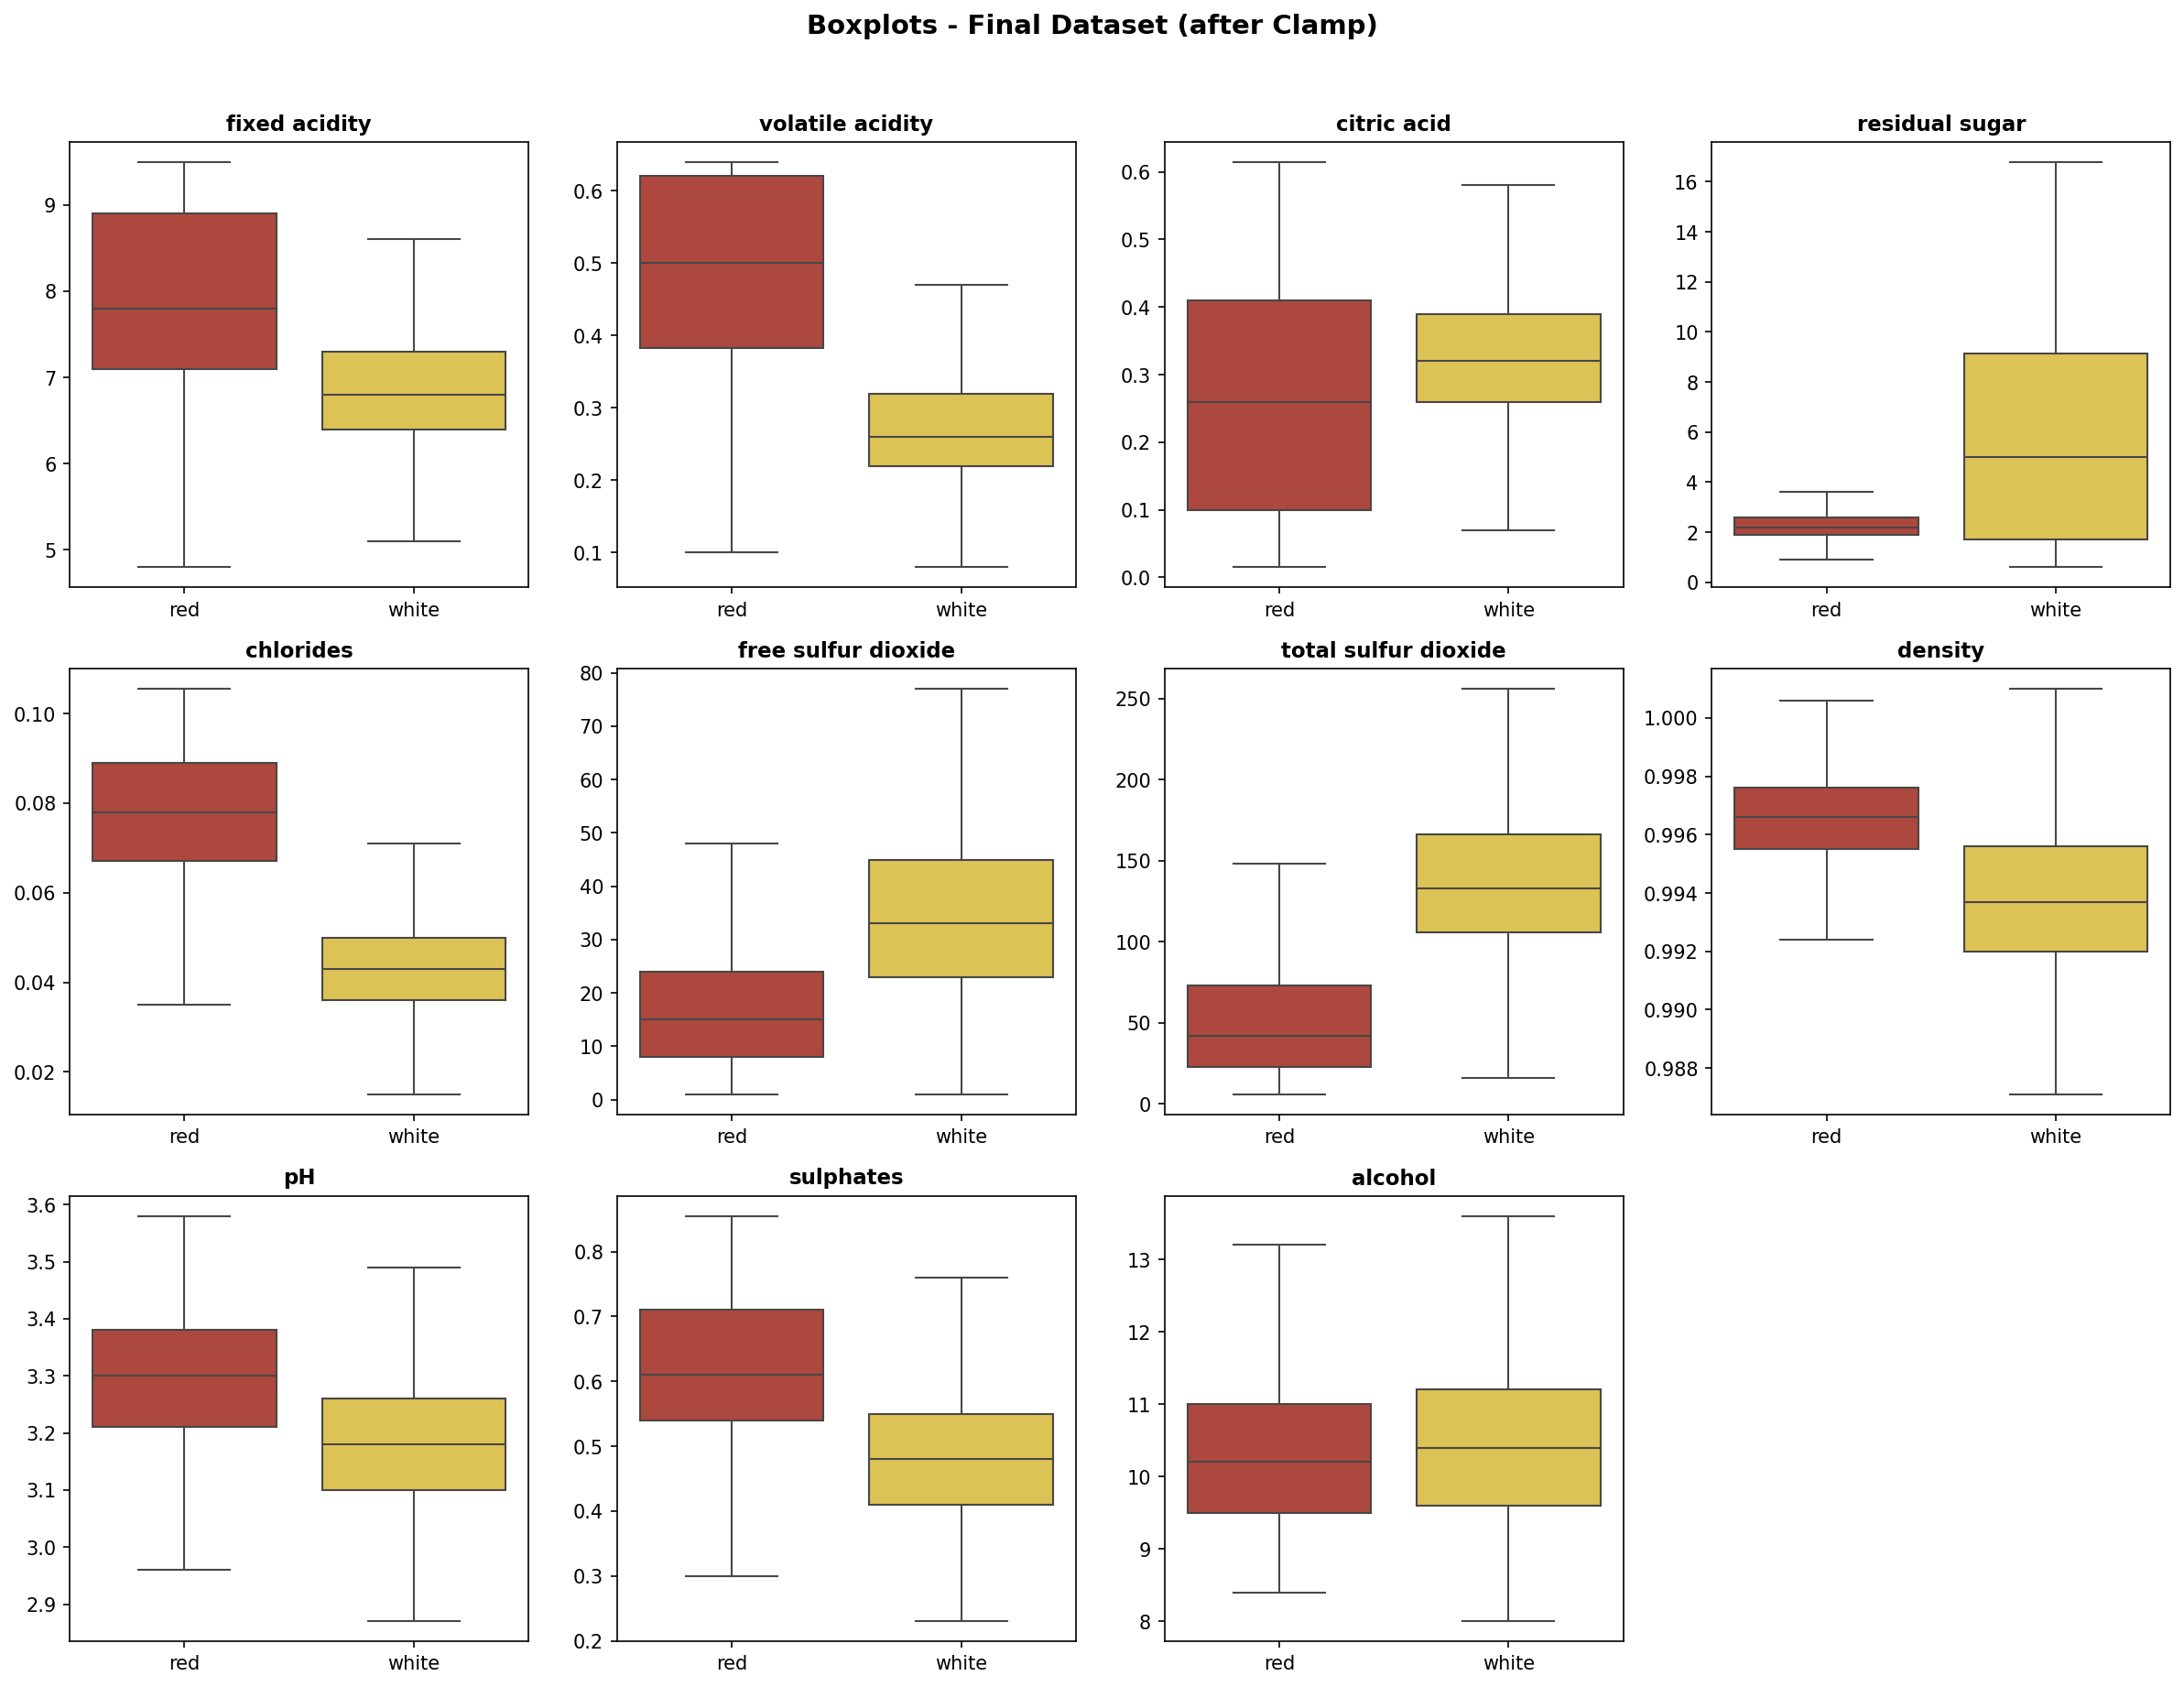
\includegraphics[width=0.98\textwidth]{final_boxplots.png}
\caption{Boxplots Συνεχών Μεταβλητών - Τελικό Dataset (μετά Clamp)}
\end{figure}

\textbf{Παρατηρήσεις:}
\begin{itemize}
    \item Μετά τον Clamp μετασχηματισμό, τα boxplots \textbf{δεν εμφανίζουν outliers} (οι ακραίες τιμές έχουν αντικατασταθεί)
    \item Οι διαφορές μεταξύ κόκκινων και λευκών κρασιών είναι εμφανείς, ιδιαίτερα στα: volatile acidity, total sulfur dioxide, density
\end{itemize}

\subsection{Histograms με Κατανομές Πυκνότητας}

Τα histograms με καμπύλη KDE (Kernel Density Estimation) δείχνουν την πυκνότητα κατανομής κάθε μεταβλητής:

\begin{figure}[H]
\centering
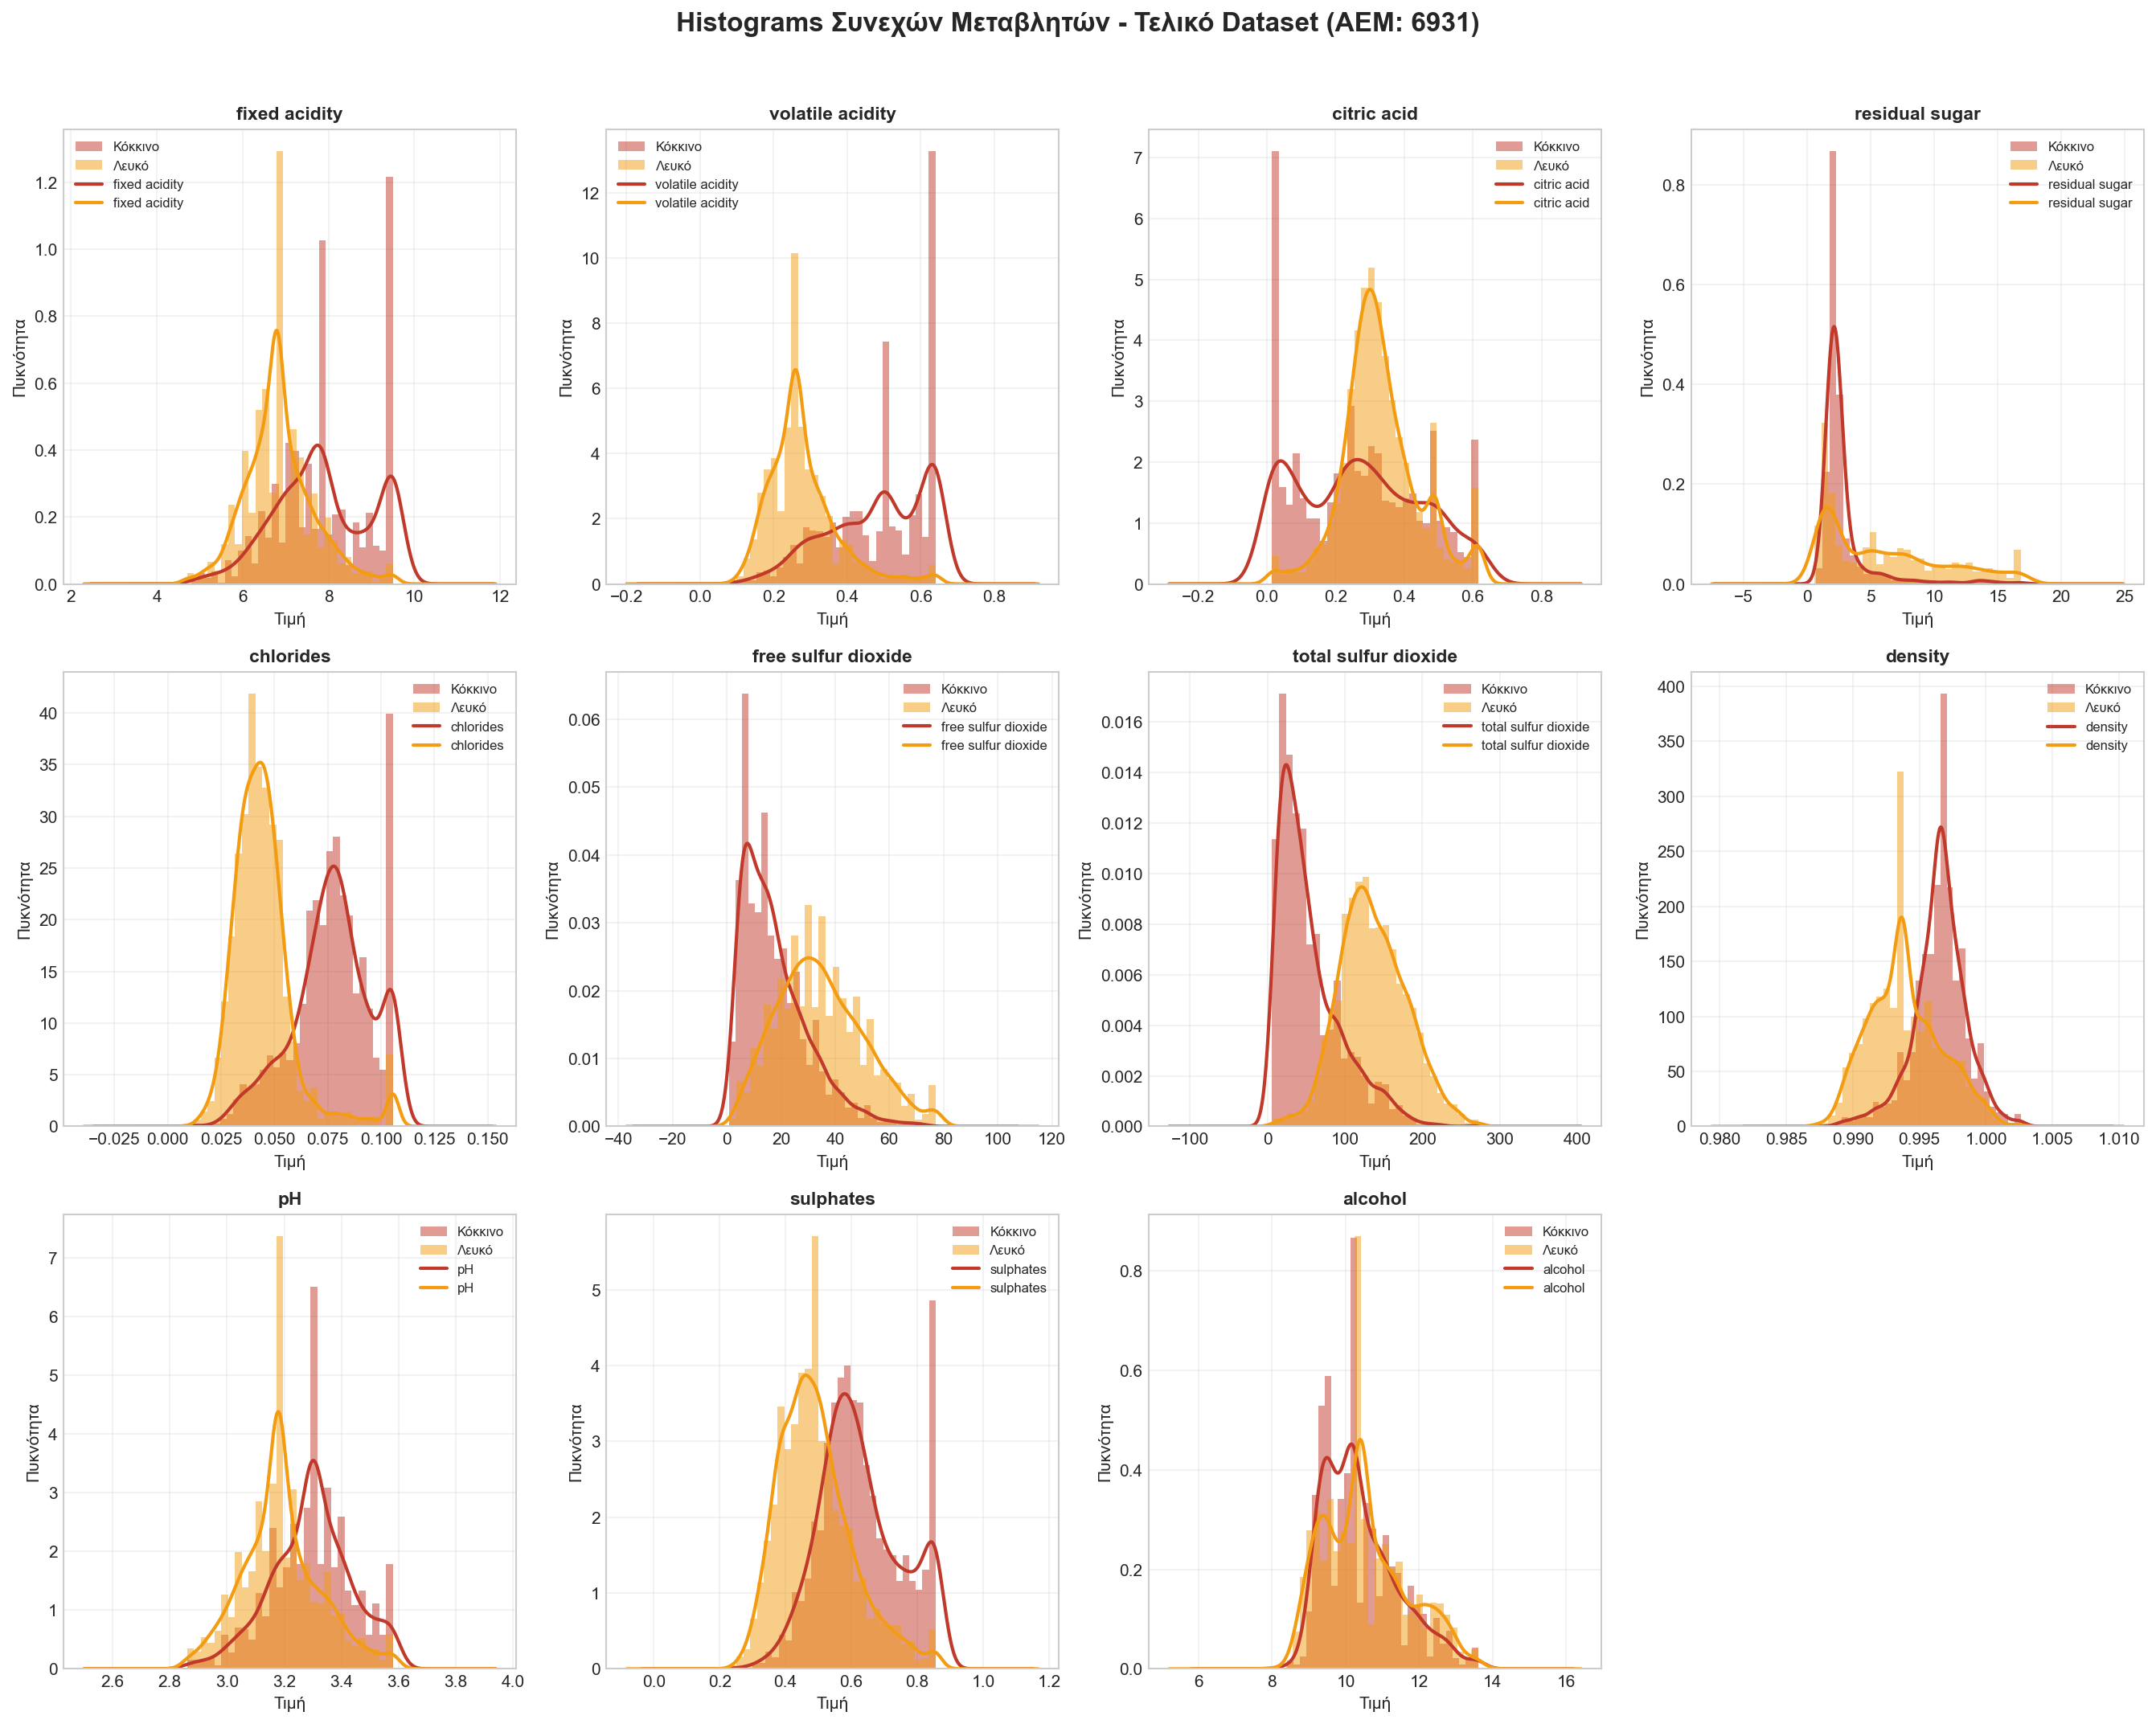
\includegraphics[width=0.98\textwidth]{final_histograms.png}
\caption{Histograms με Καμπύλη Πυκνότητας (KDE) ανά Τύπο Κρασιού}
\end{figure}

\textbf{Παρατηρήσεις:}
\begin{itemize}
    \item Τα \textbf{λευκά κρασιά} (κίτρινο) κυριαρχούν ποσοτικά σε κάθε σχήμα
    \item Ορισμένες μεταβλητές έχουν \textbf{διαφορετική κατανομή} μεταξύ τύπων κρασιού:
    \begin{itemize}
        \item \textbf{Volatile acidity:} Τα κόκκινα έχουν υψηλότερες τιμές
        \item \textbf{Total sulfur dioxide:} Τα λευκά έχουν πολύ υψηλότερες τιμές
        \item \textbf{Residual sugar:} Τα λευκά έχουν ευρύτερο εύρος
    \end{itemize}
    \item Μεταβλητές με σχεδόν \textbf{κανονική κατανομή}: pH, density
    \item Μεταβλητές με \textbf{θετική ασυμμετρία}: residual sugar, chlorides
\end{itemize}

\subsection{Correlation Heatmap (Πίνακας Συσχετίσεων)}

Ο πίνακας συσχετίσεων (correlation matrix) αποκαλύπτει τις γραμμικές σχέσεις μεταξύ των μεταβλητών:

\begin{figure}[H]
\centering
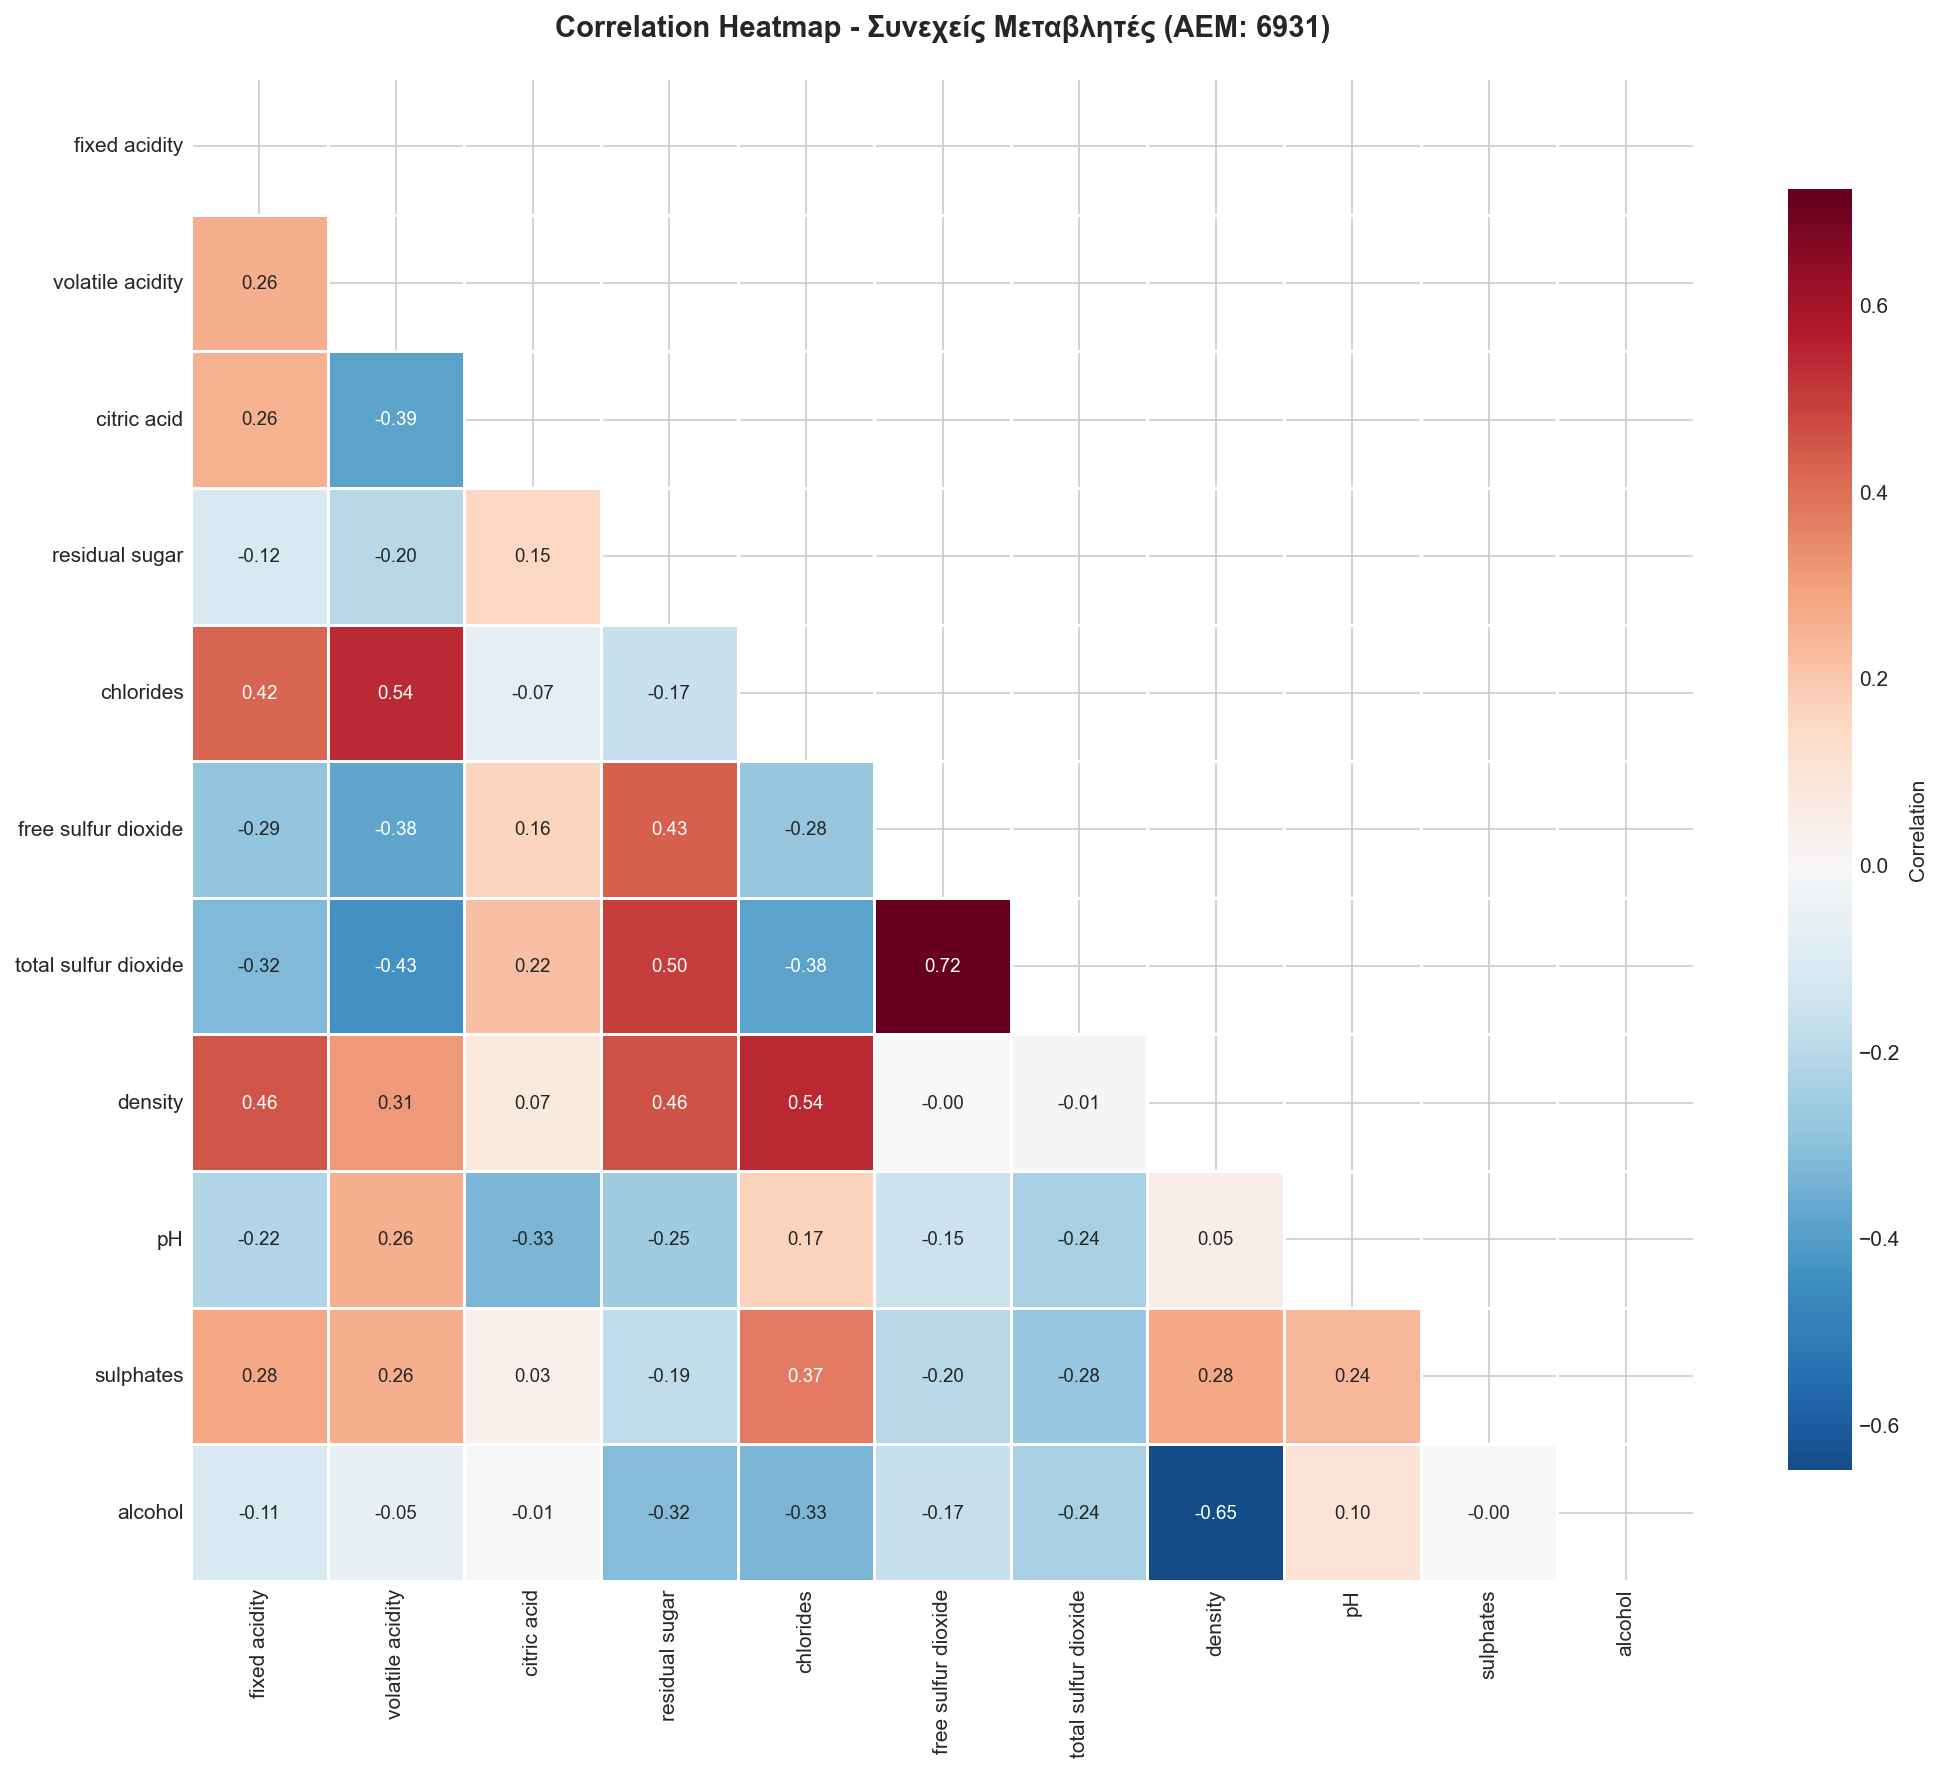
\includegraphics[width=0.85\textwidth]{correlation_heatmap.png}
\caption{Correlation Heatmap - Συντελεστές Pearson μεταξύ Συνεχών Μεταβλητών}
\end{figure}

\textbf{Ισχυρές Συσχετίσεις ($|r| > 0.5$):}

\begin{table}[H]
\centering
\caption{Ισχυρές Συσχετίσεις μεταξύ Μεταβλητών}
\begin{tabular}{llrl}
\toprule
\textbf{Μεταβλητή 1} & \textbf{Μεταβλητή 2} & \textbf{r} & \textbf{Ερμηνεία} \\
\midrule
free SO$_2$ & total SO$_2$ & +0.72 & Θετική (αναμενόμενη) \\
density & alcohol & -0.65 & Αρνητική (φυσική σχέση) \\
chlorides & density & +0.54 & Θετική \\
volatile acidity & chlorides & +0.54 & Θετική \\
residual sugar & total SO$_2$ & +0.50 & Θετική \\
\bottomrule
\end{tabular}
\end{table}

\textbf{Ερμηνεία:}
\begin{itemize}
    \item Η ισχυρότερη θετική συσχέτιση είναι μεταξύ \textbf{free και total SO$_2$} ($r = 0.72$), πράγμα λογικό αφού το ελεύθερο SO$_2$ αποτελεί μέρος του συνολικού
    \item Η ισχυρότερη αρνητική συσχέτιση είναι μεταξύ \textbf{density και alcohol} ($r = -0.65$): τα κρασιά με υψηλότερο αλκοόλ έχουν χαμηλότερη πυκνότητα (το αλκοόλ είναι ελαφρύτερο από το νερό)
    \item Η συσχέτιση \textbf{volatile acidity - chlorides} ($r = 0.54$) μπορεί να σχετίζεται με διαδικασίες ζύμωσης
\end{itemize}

\subsection{Scatter Plots Ισχυρών Συσχετίσεων}

\begin{figure}[H]
\centering
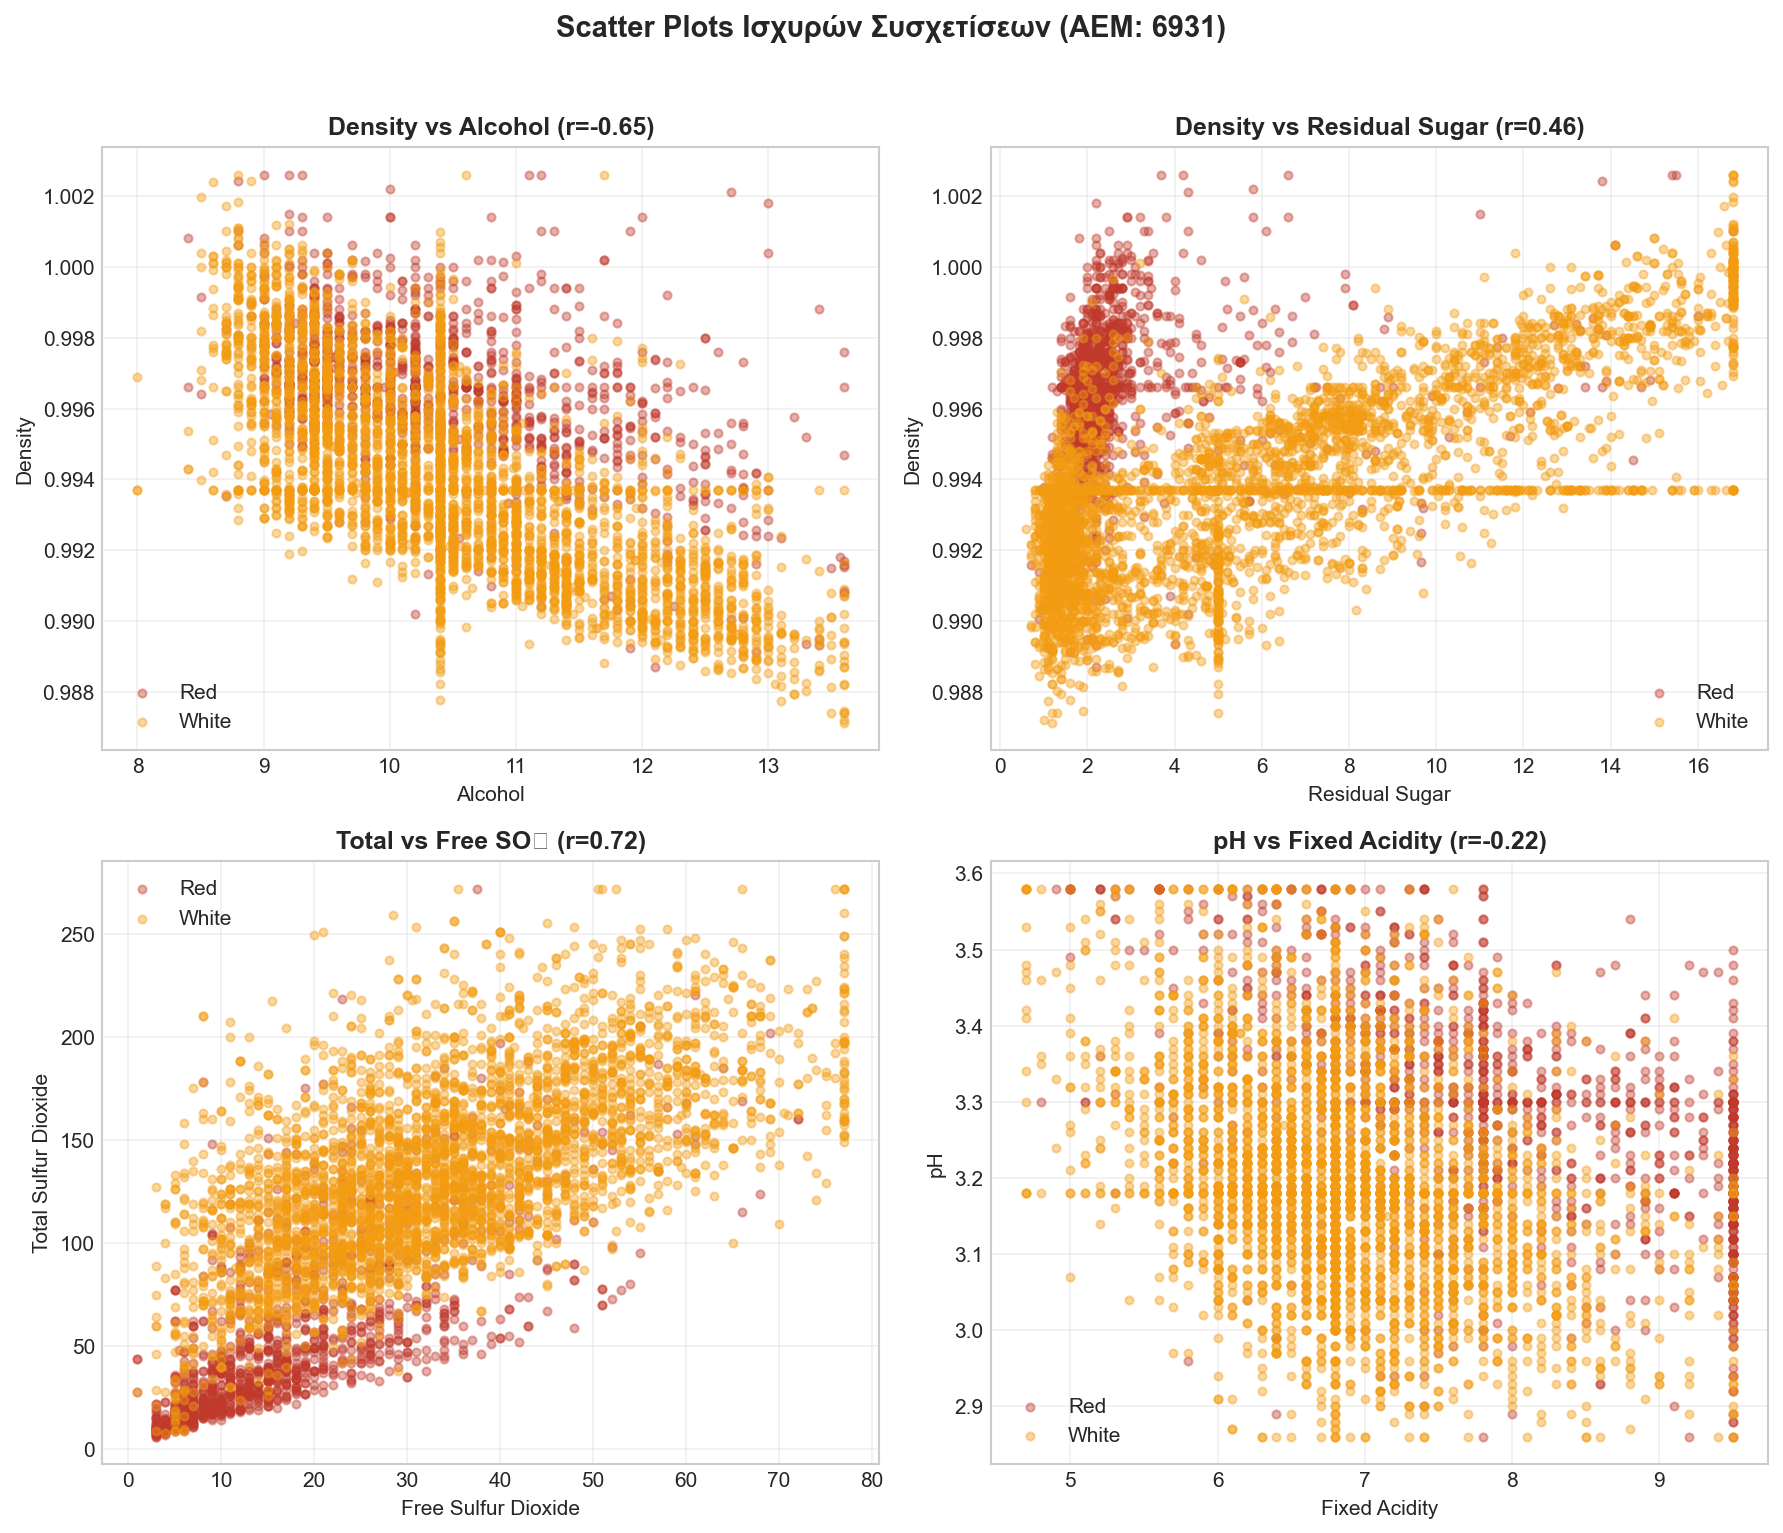
\includegraphics[width=0.95\textwidth]{scatter_correlations.png}
\caption{Scatter Plots των Ζευγαριών με τις Ισχυρότερες Συσχετίσεις}
\end{figure}

Τα scatter plots επιβεβαιώνουν οπτικά τις συσχετίσεις:
\begin{itemize}
    \item \textbf{Density vs Alcohol:} Σαφής αρνητική γραμμική τάση
    \item \textbf{Density vs Residual Sugar:} Θετική τάση, ιδιαίτερα έντονη στα λευκά κρασιά
    \item \textbf{Total vs Free SO$_2$:} Ισχυρή θετική γραμμική σχέση
    \item \textbf{pH vs Fixed Acidity:} Αρνητική τάση (υψηλή οξύτητα → χαμηλό pH)
\end{itemize}

\subsection{Violin Plots}

Τα violin plots συνδυάζουν την πληροφορία του boxplot με την κατανομή πυκνότητας:

\begin{figure}[H]
\centering
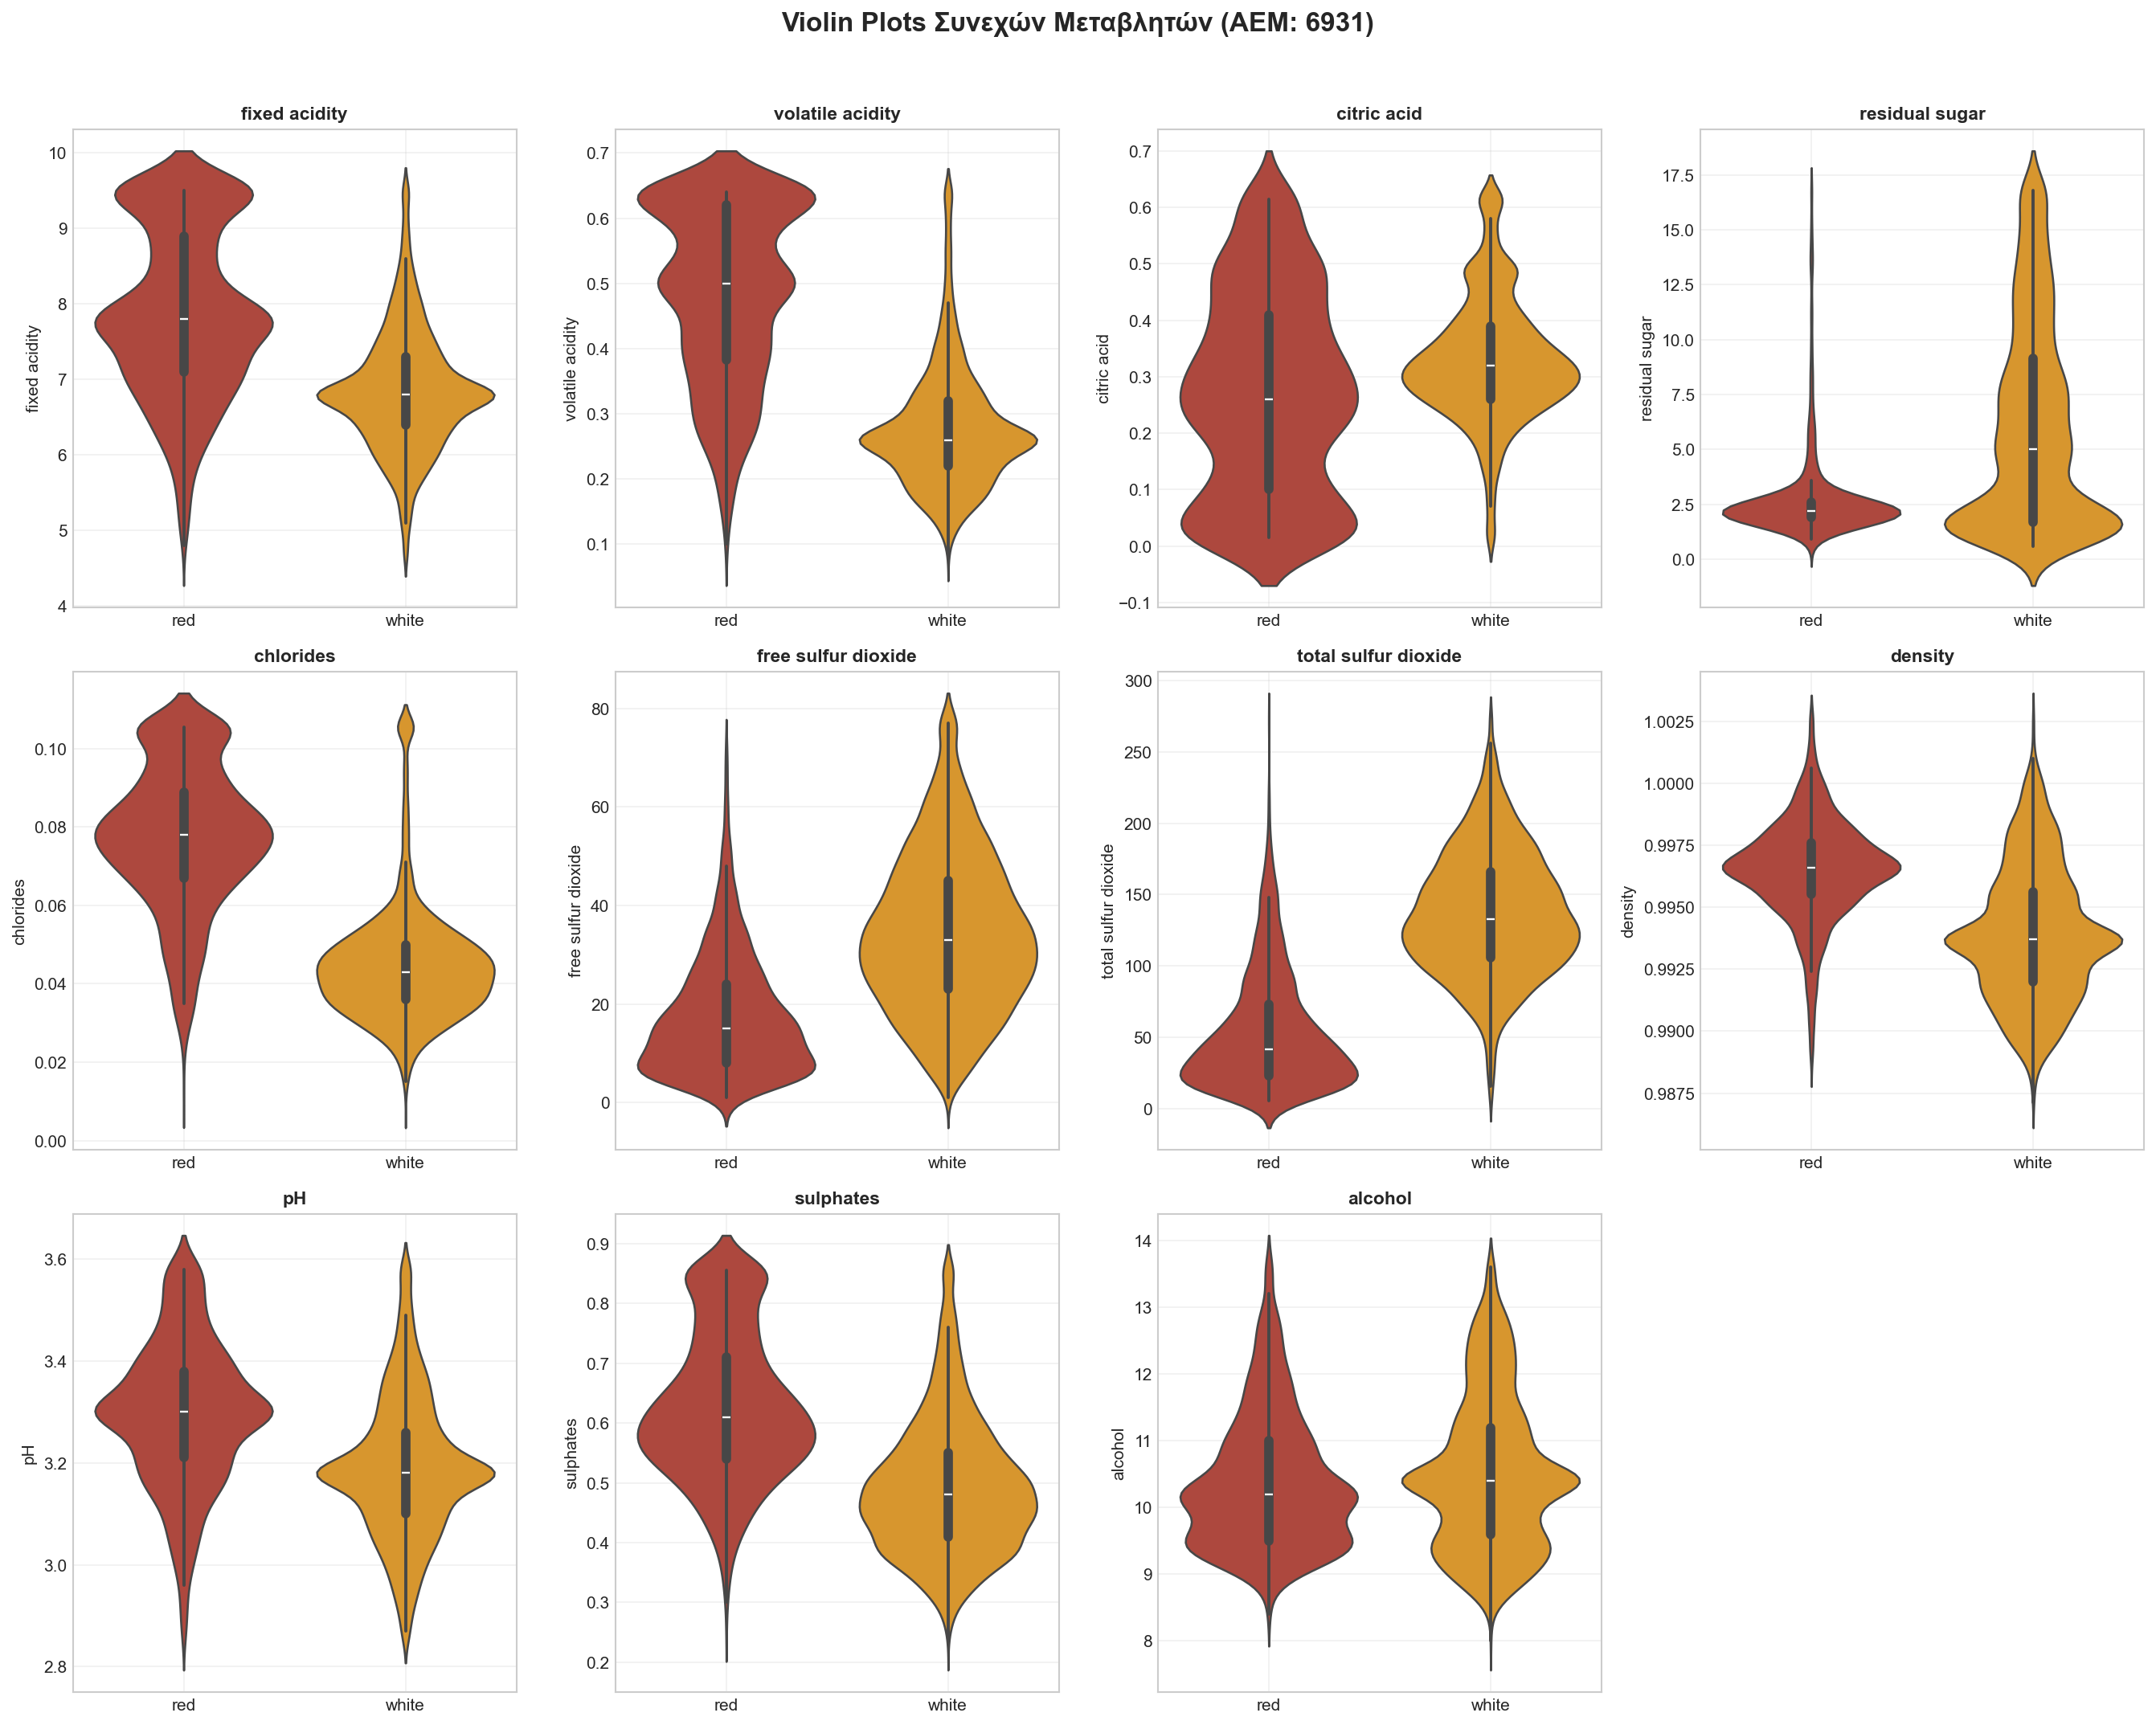
\includegraphics[width=0.98\textwidth]{violin_plots.png}
\caption{Violin Plots - Κατανομή και Πυκνότητα ανά Τύπο Κρασιού}
\end{figure}

\subsection{Συνοπτικό Dashboard}

\begin{figure}[H]
\centering
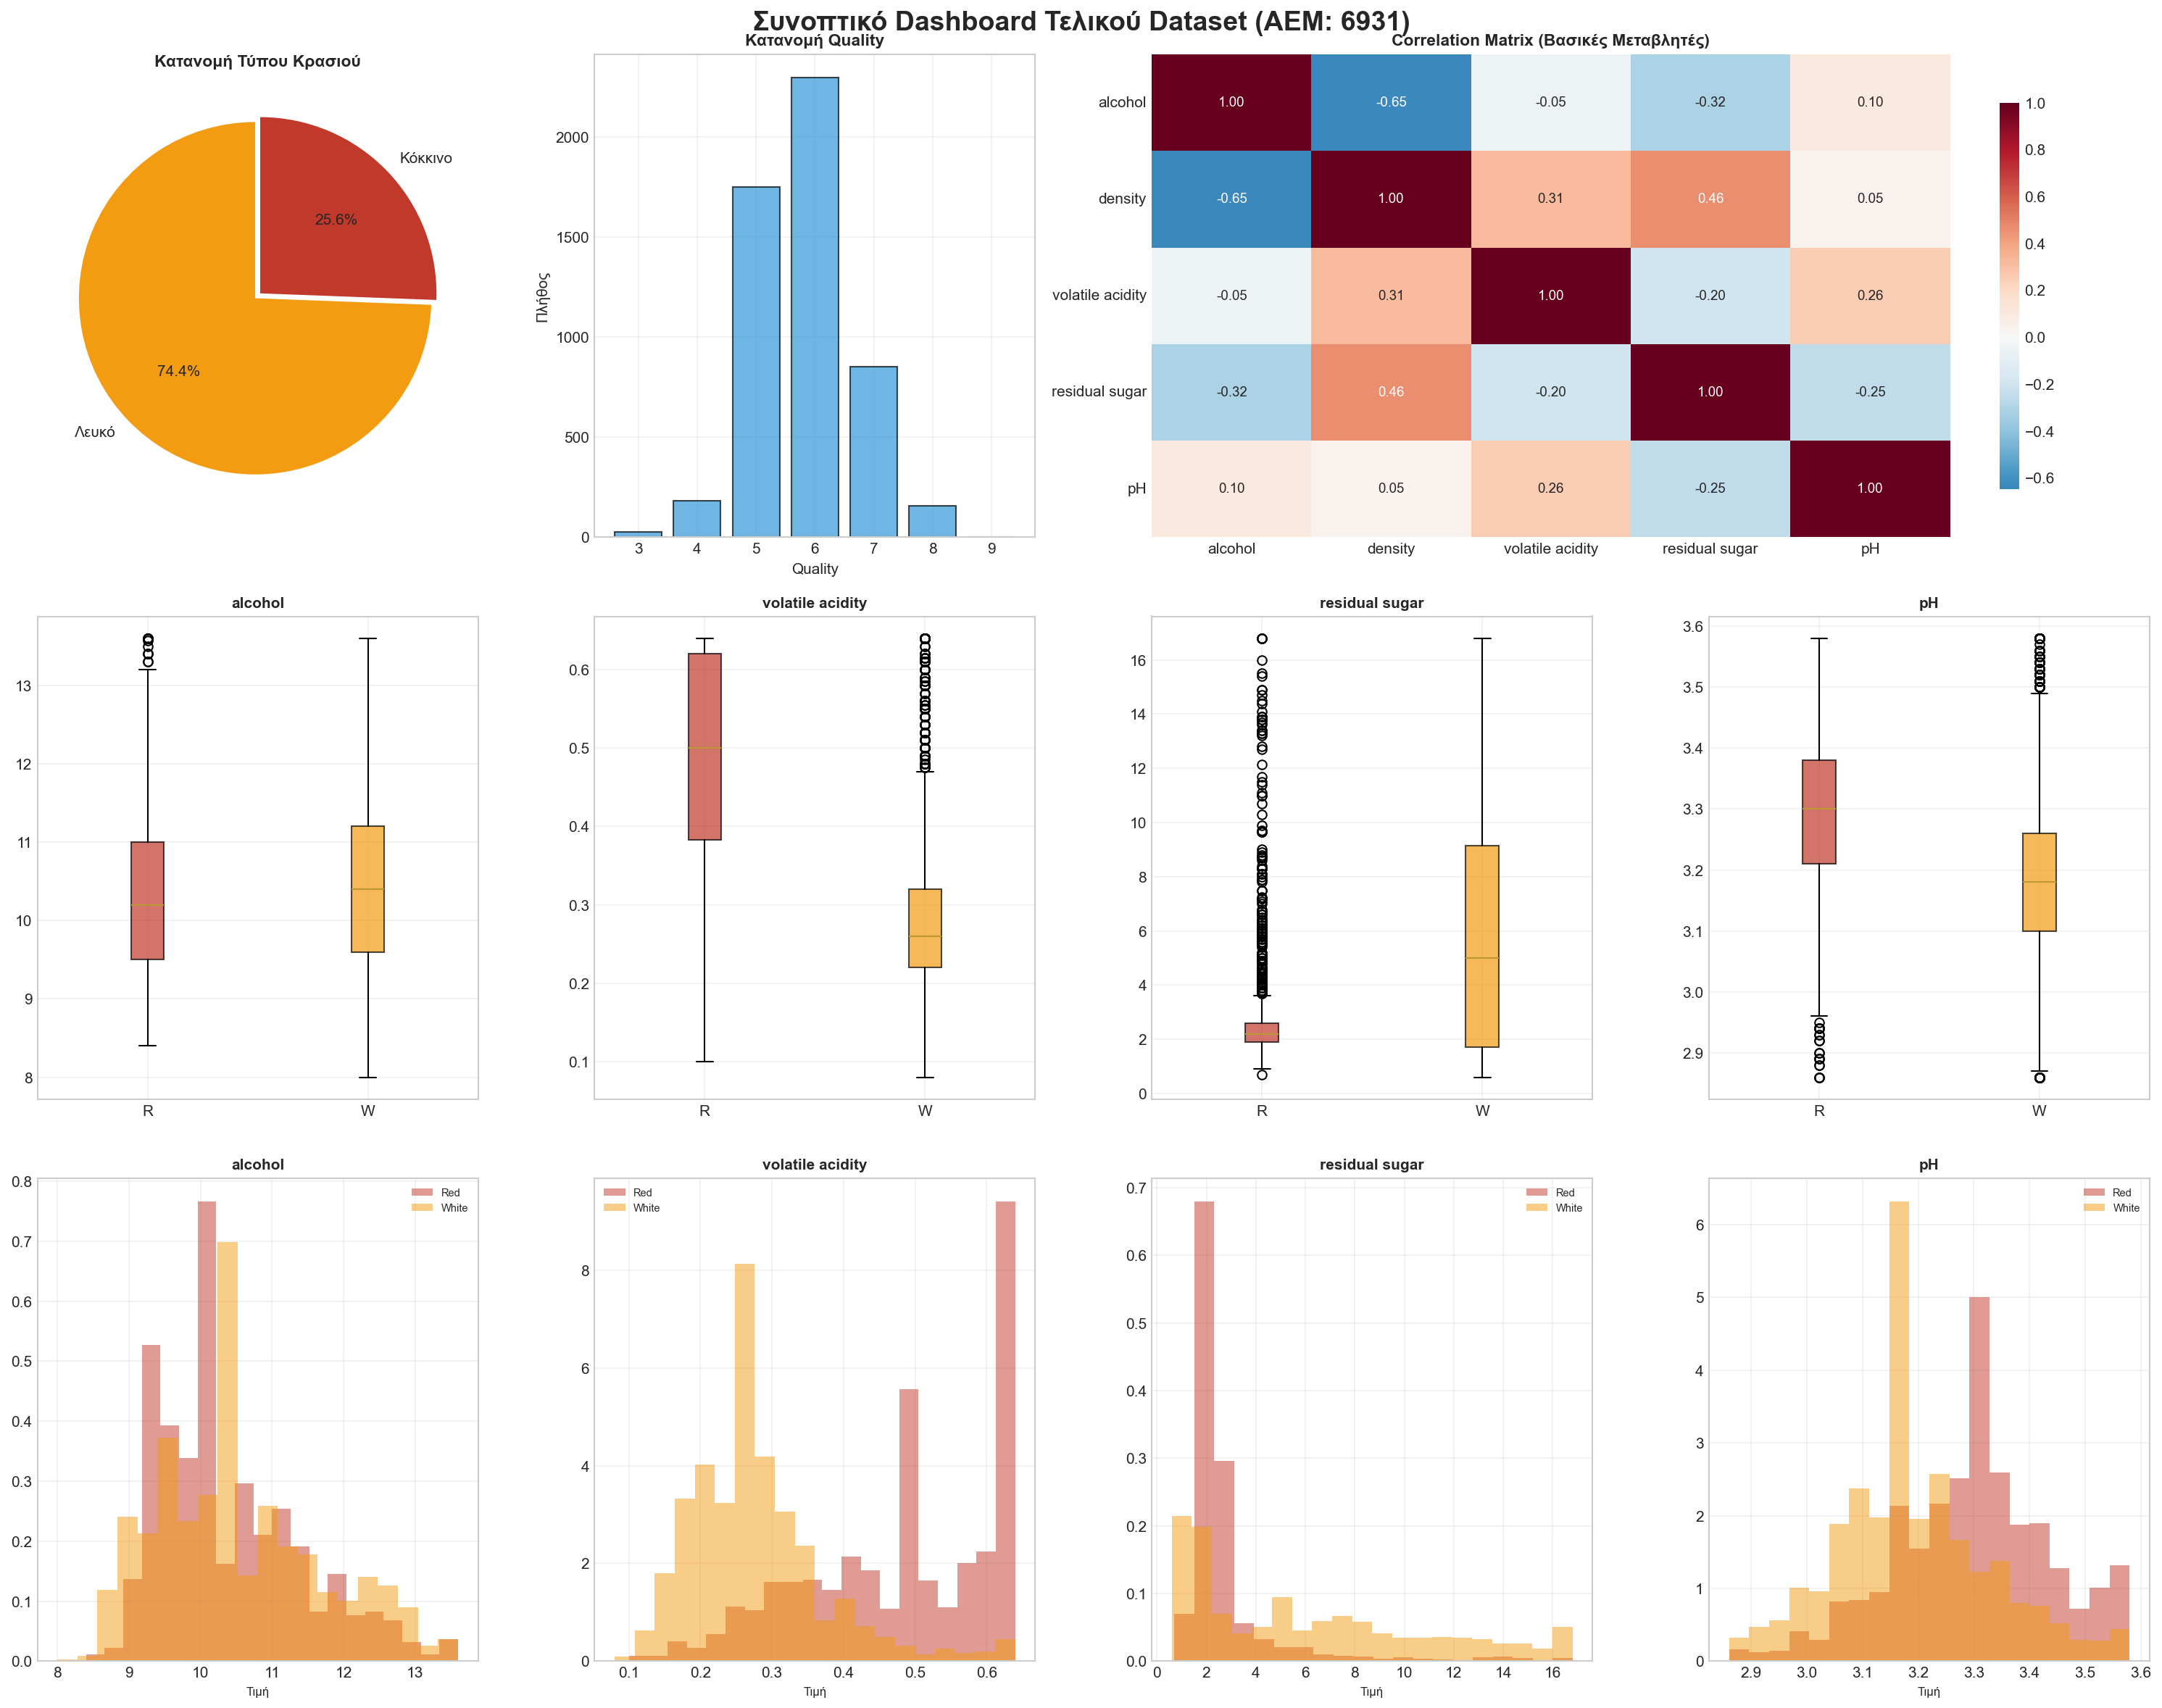
\includegraphics[width=0.98\textwidth]{summary_dashboard.png}
\caption{Συνοπτικό Dashboard του Τελικού Dataset}
\end{figure}

\subsection{Συμπεράσματα Ερωτήματος 4}

\begin{enumerate}
    \item Το τελικό dataset περιλαμβάνει \textbf{5.274 εγγραφές} και \textbf{13 μεταβλητές} (11 συνεχείς + 2 κατηγορικές)
    
    \item Τα \textbf{λευκά κρασιά αποτελούν το 74.4\%} του δείγματος, τα κόκκινα το 25.6\%
    
    \item Η πιθανότερη βαθμολογία ποιότητας είναι \textbf{6} (43.6\% των κρασιών)
    
    \item Οι πιο ισχυρές συσχετίσεις είναι:
    \begin{itemize}
        \item Free SO$_2$ ↔ Total SO$_2$ (θετική, $r = 0.72$)
        \item Density ↔ Alcohol (αρνητική, $r = -0.65$)
    \end{itemize}
    
    \item Οι κατανομές είναι \textbf{χωρίς outliers} μετά τον Clamp μετασχηματισμό
    
    \item Υπάρχουν σαφείς \textbf{διαφορές μεταξύ κόκκινων και λευκών κρασιών} σε πολλές μεταβλητές, ιδιαίτερα στα: volatile acidity, total sulfur dioxide, residual sugar
\end{enumerate}

\newpage
\appendix
\section{Πλήρης Κώδικας Python}

\subsection{Κώδικας Ερωτήματος Α: Δειγματοληψία και Καθαρισμός}

\begin{lstlisting}
import pandas as pd
import numpy as np

# Load data
df = pd.read_csv('Data Analysis_2026 1st Case_Data.csv')

# Remove unnamed columns
unnamed = [c for c in df.columns if 'Unnamed' in c]
df = df.drop(columns=unnamed)

# Sample 80%
AEM = 6931
df = df.sample(frac=0.80, random_state=AEM)
df = df.reset_index(drop=True)
print(f"After sampling: {len(df)} rows")

# Fix wine_type typos
fixes = {
    'Redd ':'red', 'r3d':'red', 
    'WHITTE':'white', 'whit':'white', 'whate':'white',
    '999':np.nan, '9999':np.nan, '-999':np.nan, '?':np.nan
}
for wrong, correct in fixes.items():
    df.loc[df['wine_type']==wrong, 'wine_type'] = correct

# Convert numeric columns
num_cols = ['fixed acidity', 'volatile acidity', 
            'citric acid', 'residual sugar', 'chlorides', 
            'free sulfur dioxide', 'total sulfur dioxide',
            'density', 'pH', 'sulphates', 'alcohol', 'quality']

for col in num_cols:
    df[col] = pd.to_numeric(df[col], errors='coerce')

# Replace impossible values with NaN
limits = {
    'fixed acidity': (0, 20),
    'volatile acidity': (0, 5),
    'citric acid': (0, 3),
    'residual sugar': (0, 100),
    'chlorides': (0, 1),
    'free sulfur dioxide': (0, 300),
    'total sulfur dioxide': (0, 500),
    'density': (0.9, 1.1),
    'pH': (2, 5),
    'sulphates': (0, 3),
    'alcohol': (5, 20),
    'quality': (0, 10)
}

for col, (min_val, max_val) in limits.items():
    mask = (df[col] < min_val) | (df[col] > max_val)
    df.loc[mask, col] = np.nan

# Remove duplicates
df = df.drop_duplicates().reset_index(drop=True)
print(f"After removing duplicates: {len(df)} rows")

# Fill missing values with median by wine type
df['wine_type'].fillna(df['wine_type'].mode()[0], inplace=True)

for col in num_cols:
    for wine in ['red', 'white']:
        mask = (df['wine_type'] == wine) & (df[col].isna())
        median = df.loc[df['wine_type'] == wine, col].median()
        df.loc[mask, col] = median

# Verify no missing values
print(f"Missing values: {df.isna().sum().sum()}")
print(f"Final shape: {df.shape}")

# Save cleaned data
df.to_csv('cleaned_wine_data_AEM_6931.csv', index=False)
print("Saved to cleaned_wine_data_AEM_6931.csv")
\end{lstlisting}

\subsection{Κώδικας Ερωτήματος Β: Boxplots και Κατανομή Quality}

\begin{lstlisting}
import pandas as pd
import numpy as np
import matplotlib.pyplot as plt
from matplotlib.patches import Patch

# Load cleaned data
AEM = 6931
df = pd.read_csv(f'cleaned_wine_data_AEM_{AEM}.csv')

# Continuous variables (excluding quality - it's discrete)
continuous_vars = ['fixed acidity', 'volatile acidity', 'citric acid',
                   'residual sugar', 'chlorides', 'free sulfur dioxide',
                   'total sulfur dioxide', 'density', 'pH', 'sulphates',
                   'alcohol']

colors = {'all': '#3498db', 'red': '#e74c3c', 'white': '#f1c40f'}

# ============================================================
# Boxplots for all data (11 continuous variables)
# ============================================================
fig, axes = plt.subplots(3, 4, figsize=(16, 12))
fig.suptitle('Boxplots Συνεχών Μεταβλητών - Σύνολο Δεδομένων (ΑΕΜ: 6931)',
             fontsize=14, fontweight='bold')

for idx, var in enumerate(continuous_vars):
    row = idx // 4
    col = idx % 4
    ax = axes[row, col]

    bp = ax.boxplot(df[var].dropna(), patch_artist=True)
    bp['boxes'][0].set_facecolor(colors['all'])
    bp['boxes'][0].set_alpha(0.7)

    ax.set_title(var, fontsize=10, fontweight='bold')
    ax.set_ylabel('Τιμή')
    ax.grid(True, alpha=0.3)

plt.tight_layout()
plt.savefig('boxplots_all_data.png', dpi=150, bbox_inches='tight')
plt.close()

# ============================================================
# Quality Distribution (Discrete Variable)
# ============================================================
fig, axes = plt.subplots(1, 2, figsize=(14, 5))
fig.suptitle('Κατανομή Quality (Διακριτή Μεταβλητή) - ΑΕΜ: 6931', 
             fontsize=14, fontweight='bold')

# Overall distribution
quality_counts = df['quality'].value_counts().sort_index()
axes[0].bar(quality_counts.index, quality_counts.values, color=colors['all'], 
            alpha=0.7, edgecolor='black')
axes[0].set_title('Συνολική Κατανομή', fontweight='bold')
axes[0].set_xlabel('Quality Score')
axes[0].set_ylabel('Συχνότητα')
axes[0].grid(True, alpha=0.3, axis='y')

# Distribution by wine type
quality_red = df[df['wine_type'] == 'red']['quality'].value_counts().sort_index()
quality_white = df[df['wine_type'] == 'white']['quality'].value_counts().sort_index()

x = np.arange(len(quality_counts.index))
width = 0.35

axes[1].bar(x - width/2, [quality_red.get(i, 0) for i in quality_counts.index], 
            width, label='Κόκκινο', color=colors['red'], alpha=0.7, edgecolor='black')
axes[1].bar(x + width/2, [quality_white.get(i, 0) for i in quality_counts.index], 
            width, label='Λευκό', color=colors['white'], alpha=0.7, edgecolor='black')
axes[1].set_title('Σύγκριση: Κόκκινο vs Λευκό', fontweight='bold')
axes[1].set_xlabel('Quality Score')
axes[1].set_ylabel('Συχνότητα')
axes[1].set_xticks(x)
axes[1].set_xticklabels(quality_counts.index)
axes[1].legend()
axes[1].grid(True, alpha=0.3, axis='y')

plt.tight_layout()
plt.savefig('quality_distribution.png', dpi=150, bbox_inches='tight')
plt.close()

# ============================================================
# Boxplots by Wine Type
# ============================================================
df_red = df[df['wine_type'] == 'red']
df_white = df[df['wine_type'] == 'white']

fig, axes = plt.subplots(3, 4, figsize=(18, 12))
fig.suptitle('Boxplots Συνεχών Μεταβλητών - Σύγκριση Κόκκινου vs Λευκού (ΑΕΜ: 6931)',
             fontsize=14, fontweight='bold')

for idx, var in enumerate(continuous_vars):
    row = idx // 4
    col = idx % 4
    ax = axes[row, col]

    data_to_plot = [df_red[var].dropna(), df_white[var].dropna()]
    bp = ax.boxplot(data_to_plot, patch_artist=True, labels=['Κόκκινο', 'Λευκό'])

    bp['boxes'][0].set_facecolor(colors['red'])
    bp['boxes'][1].set_facecolor(colors['white'])
    for box in bp['boxes']:
        box.set_alpha(0.7)

    ax.set_title(var, fontsize=10, fontweight='bold')
    ax.set_ylabel('Τιμή')
    ax.grid(True, alpha=0.3)

legend_elements = [Patch(facecolor=colors['red'], alpha=0.7, label='Κόκκινο'),
                   Patch(facecolor=colors['white'], alpha=0.7, label='Λευκό')]
fig.legend(handles=legend_elements, loc='lower right', fontsize=11)

plt.tight_layout()
plt.savefig('boxplots_by_wine_type.png', dpi=150, bbox_inches='tight')
plt.close()

print('Saved: boxplots_all_data.png')
print('Saved: quality_distribution.png')
print('Saved: boxplots_by_wine_type.png')
\end{lstlisting}

\subsection{Κώδικας Ερωτήματος Γ: Εντοπισμός Ακραίων Τιμών και Clamp Transformation}

\begin{lstlisting}
import pandas as pd
import matplotlib.pyplot as plt
from matplotlib.patches import Patch

# Load cleaned data
AEM = 6931
df = pd.read_csv(f'cleaned_wine_data_AEM_{AEM}.csv')

continuous_vars = ['fixed acidity', 'volatile acidity', 'citric acid',
                   'residual sugar', 'chlorides', 'free sulfur dioxide',
                   'total sulfur dioxide', 'density', 'pH', 'sulphates',
                   'alcohol', 'quality']

# Copy for transformation
df_transformed = df.copy()

# ============================================================
# IQR Method
# ============================================================
iqr_outliers = {}
iqr_bounds = {}

for var in continuous_vars:
    Q1 = df[var].quantile(0.25)
    Q3 = df[var].quantile(0.75)
    IQR = Q3 - Q1

    lower_bound = Q1 - 1.5 * IQR
    upper_bound = Q3 + 1.5 * IQR

    outliers_mask = (df[var] < lower_bound) | (df[var] > upper_bound)
    n_outliers = outliers_mask.sum()

    iqr_outliers[var] = n_outliers
    iqr_bounds[var] = (lower_bound, upper_bound)

    print(f"{var}: {n_outliers} outliers "
          f"[{lower_bound:.4f}, {upper_bound:.4f}]")

print(f"Total IQR outliers: {sum(iqr_outliers.values())}")

# ============================================================
# Z-Score Method (threshold = 3.5)
# ============================================================
zscore_outliers = {}
z_threshold = 3.5

for var in continuous_vars:
    mean = df[var].mean()
    std = df[var].std()

    lower_bound = mean - z_threshold * std
    upper_bound = mean + z_threshold * std

    outliers_mask = (df[var] < lower_bound) | (df[var] > upper_bound)
    n_outliers = outliers_mask.sum()

    zscore_outliers[var] = n_outliers

    print(f"{var}: {n_outliers} outliers "
          f"[{lower_bound:.4f}, {upper_bound:.4f}]")

print(f"Total Z-score outliers: {sum(zscore_outliers.values())}")

# ============================================================
# Clamp Transformation (based on IQR bounds)
# ============================================================
for var in continuous_vars:
    lower_bound, upper_bound = iqr_bounds[var]
    df_transformed[var] = df_transformed[var].clip(
        lower=lower_bound, upper=upper_bound)

# ============================================================
# Boxplots Before and After Clamp
# ============================================================
fig, axes = plt.subplots(3, 4, figsize=(18, 14))
fig.suptitle('Boxplots BEFORE (blue) and AFTER (green) '
             'Clamp Transformation (AEM: 6931)',
             fontsize=14, fontweight='bold')

for idx, var in enumerate(continuous_vars):
    row = idx // 4
    col = idx % 4
    ax = axes[row, col]

    data_before = df[var].dropna()
    data_after = df_transformed[var].dropna()

    bp = ax.boxplot([data_before, data_after],
                    patch_artist=True,
                    labels=['Before', 'After'])

    bp['boxes'][0].set_facecolor('#3498db')
    bp['boxes'][1].set_facecolor('#2ecc71')
    for box in bp['boxes']:
        box.set_alpha(0.7)

    ax.set_title(var, fontsize=10, fontweight='bold')
    ax.set_ylabel('Value')
    ax.grid(True, alpha=0.3)

legend_elements = [
    Patch(facecolor='#3498db', alpha=0.7, label='Before Clamp'),
    Patch(facecolor='#2ecc71', alpha=0.7, label='After Clamp')]
fig.legend(handles=legend_elements, loc='lower right',
           fontsize=11)

plt.tight_layout()
plt.savefig('boxplots_before_after_clamp.png',
            dpi=150, bbox_inches='tight')
plt.close()

# Save transformed data
output_file = f'transformed_wine_data_AEM_{AEM}.csv'
df_transformed.to_csv(output_file, index=False)
print(f'Saved: {output_file}')
\end{lstlisting}

\subsection{Κώδικας Ερωτήματος Δ: Οπτική Παρουσίαση και Περιγραφικά Στατιστικά}

\begin{lstlisting}
import pandas as pd
import numpy as np
import matplotlib.pyplot as plt
import seaborn as sns

# Load transformed data
AEM = 6931
df = pd.read_csv(f'transformed_wine_data_AEM_{AEM}.csv')

# Define variables
continuous_vars = ['fixed acidity', 'volatile acidity', 'citric acid',
                   'residual sugar', 'chlorides', 'free sulfur dioxide',
                   'total sulfur dioxide', 'density', 'pH', 'sulphates',
                   'alcohol']
categorical_vars = ['wine_type', 'quality']
colors = {'red': '#c0392b', 'white': '#f39c12', 'all': '#3498db'}

# ============================================================
# 1. Descriptive Statistics - Continuous Variables
# ============================================================
continuous_stats = pd.DataFrame()
for var in continuous_vars:
    stats = {
        'Variable': var,
        'N': df[var].count(),
        'Missing': df[var].isna().sum(),
        'Mean': df[var].mean(),
        'Median': df[var].median(),
        'Std': df[var].std(),
        'Min': df[var].min(),
        'Max': df[var].max(),
        'Q1': df[var].quantile(0.25),
        'Q3': df[var].quantile(0.75),
        'IQR': df[var].quantile(0.75) - df[var].quantile(0.25),
        'Skewness': df[var].skew(),
        'Cardinality': df[var].nunique()
    }
    continuous_stats = pd.concat([continuous_stats,
                                   pd.DataFrame([stats])],
                                  ignore_index=True)
continuous_stats.to_csv('descriptive_stats_continuous.csv', index=False)

# ============================================================
# 2. Descriptive Statistics - Categorical Variables
# ============================================================
categorical_stats = pd.DataFrame()
for var in categorical_vars:
    value_counts = df[var].value_counts()
    stats = {
        'Variable': var,
        'N': df[var].count(),
        'Missing': df[var].isna().sum(),
        'Cardinality': df[var].nunique(),
        'Mode': df[var].mode()[0],
        'Mode_Freq': value_counts.iloc[0],
        'Mode_Pct': (value_counts.iloc[0] / len(df)) * 100
    }
    categorical_stats = pd.concat([categorical_stats,
                                    pd.DataFrame([stats])],
                                   ignore_index=True)
categorical_stats.to_csv('descriptive_stats_categorical.csv', index=False)

# ============================================================
# 3. Boxplots (Final Dataset)
# ============================================================
fig, axes = plt.subplots(3, 4, figsize=(18, 14))
fig.suptitle('Boxplots - Final Dataset (AEM: 6931)',
             fontsize=16, fontweight='bold')
df_red = df[df['wine_type'] == 'red']
df_white = df[df['wine_type'] == 'white']

for idx, var in enumerate(continuous_vars):
    ax = axes[idx // 4, idx % 4]
    bp = ax.boxplot([df_red[var], df_white[var]],
                    patch_artist=True, labels=['Red', 'White'])
    bp['boxes'][0].set_facecolor(colors['red'])
    bp['boxes'][1].set_facecolor(colors['white'])
    ax.set_title(var, fontweight='bold')
    ax.grid(True, alpha=0.3)
axes[2, 3].axis('off')
plt.tight_layout()
plt.savefig('final_boxplots.png', dpi=150, bbox_inches='tight')
plt.close()

# ============================================================
# 4. Histograms with KDE
# ============================================================
fig, axes = plt.subplots(3, 4, figsize=(18, 14))
fig.suptitle('Histograms with KDE (AEM: 6931)',
             fontsize=16, fontweight='bold')

for idx, var in enumerate(continuous_vars):
    ax = axes[idx // 4, idx % 4]
    ax.hist(df_red[var], bins=30, alpha=0.5, label='Red',
            color=colors['red'], density=True)
    ax.hist(df_white[var], bins=30, alpha=0.5, label='White',
            color=colors['white'], density=True)
    df_red[var].plot(kind='kde', ax=ax, color=colors['red'])
    df_white[var].plot(kind='kde', ax=ax, color=colors['white'])
    ax.set_title(var, fontweight='bold')
    ax.legend(fontsize=8)
    ax.grid(True, alpha=0.3)
axes[2, 3].axis('off')
plt.tight_layout()
plt.savefig('final_histograms.png', dpi=150, bbox_inches='tight')
plt.close()

# ============================================================
# 5. Correlation Heatmap
# ============================================================
corr_matrix = df[continuous_vars].corr()
plt.figure(figsize=(14, 12))
mask = np.triu(np.ones_like(corr_matrix, dtype=bool))
sns.heatmap(corr_matrix, mask=mask, annot=True, fmt='.2f',
            cmap='RdBu_r', center=0, square=True,
            linewidths=0.5, cbar_kws={'shrink': 0.8})
plt.title('Correlation Heatmap (AEM: 6931)',
          fontsize=14, fontweight='bold')
plt.tight_layout()
plt.savefig('correlation_heatmap.png', dpi=150, bbox_inches='tight')
plt.close()

# Print strong correlations
print("Strong Correlations (|r| > 0.5):")
for i in range(len(corr_matrix.columns)):
    for j in range(i+1, len(corr_matrix.columns)):
        r = corr_matrix.iloc[i, j]
        if abs(r) > 0.5:
            print(f"  {corr_matrix.columns[i]} <-> "
                  f"{corr_matrix.columns[j]}: r = {r:.3f}")

# ============================================================
# 6. Violin Plots
# ============================================================
fig, axes = plt.subplots(3, 4, figsize=(18, 14))
fig.suptitle('Violin Plots (AEM: 6931)',
             fontsize=16, fontweight='bold')

for idx, var in enumerate(continuous_vars):
    ax = axes[idx // 4, idx % 4]
    sns.violinplot(data=df, x='wine_type', y=var, ax=ax,
                   palette={'red': colors['red'],
                            'white': colors['white']},
                   inner='box')
    ax.set_title(var, fontweight='bold')
    ax.set_xlabel('')
    ax.grid(True, alpha=0.3)
axes[2, 3].axis('off')
plt.tight_layout()
plt.savefig('violin_plots.png', dpi=150, bbox_inches='tight')
plt.close()

print("All visualizations saved successfully!")
\end{lstlisting}

\end{document}
